
\documentclass[UTF8,a4paper,12pt]{ctexart}

\usepackage{geometry}
\usepackage{amsmath,amssymb}
\usepackage{booktabs,longtable,array}
\usepackage{graphicx,float}
\graphicspath{{../../problems/D/q1/figures/}{problems/D/q1/figures/}}
\usepackage{xcolor}
\usepackage{tikz}
\usetikzlibrary{arrows.meta,positioning,calc,fit,patterns,shapes.geometric}
\usepackage{enumitem}
\usepackage{caption}
\usepackage{subcaption}
\usepackage[hidelinks]{hyperref}

\geometry{left=2.6cm,right=2.6cm,top=2.5cm,bottom=2.5cm}
\setlength{\parindent}{2em}
\setlength{\parskip}{0.25em}
\renewcommand{\arraystretch}{1.18}
\setcounter{tocdepth}{2}
\setcounter{secnumdepth}{3}

\newcommand{\figplaceholder}[2][5.2cm]{%
  \begin{figure}[H]
    \centering
    \fbox{\parbox[c][#1][c]{0.92\textwidth}{\centering #2}}
  \end{figure}
}

\title{山区洪涝救援中无人机运输--通信协同调度与独立资源配置}
\author{}
\date{}

% Q2-EVIDENCE-V7-FOCUSED formal manuscript figures.
% Auto-generated from paper/data/q2_v7_visual_source.json.
% No legacy q2_closing figure is used by these macros.
\definecolor{qLight}{HTML}{E4E8EB}
\definecolor{qLMid}{HTML}{C4CDD3}
\definecolor{qMid}{HTML}{98A8B2}
\definecolor{qDark}{HTML}{657A87}
\definecolor{qDeep}{HTML}{3F5663}
\definecolor{qText}{HTML}{30343A}
\definecolor{qGrid}{HTML}{D9DDE0}

\newcommand{\QTwoFigFramework}{%
\begin{tikzpicture}[>=Latex,font=\small]
\node[draw=qDark,fill=qLight,rounded corners=2pt,minimum width=5.0cm,minimum height=.8cm,align=center] (a) at (0,4.9) {Q1安全可行批型 / 候选运输任务};
\node[draw=qDark,fill=qLight,rounded corners=2pt,minimum width=6.2cm,minimum height=1.05cm,align=center] (b) at (0,3.5) {多点运输任务构造\\箱组 · 访问顺序 · 机型 · 时长 · 能耗 · 箱级送达偏移};
\node[draw=qDark,fill=qLMid,rounded corners=2pt,minimum width=6.2cm,minimum height=1.05cm,align=center] (c) at (0,2.0) {飞机--电池联合资源排程\\实体飞机 · 共享电池 · 充电恢复 · deadline · 开始时刻};
\node[draw=qDark,fill=qLight,rounded corners=2pt,minimum width=5.2cm,minimum height=1.35cm,align=center] (u) at (-3.7,.25) {可行上界路线\\任务重构 $\to$ 事件排程 $\to$ 独立重放\\得到真实可执行 UB};
\node[draw=qDark,fill=qLight,rounded corners=2pt,minimum width=5.2cm,minimum height=1.35cm,align=center] (l) at (3.7,.25) {全局下界路线\\任务列松弛 $\to$ 完整定价 $\to$ 分支覆盖证书\\得到有效 LB};
\node[draw=qDark,fill=qLMid,rounded corners=2pt,minimum width=5.4cm,minimum height=.85cm,align=center] (z) at (0,-1.45) {确定性认证区间：$LB\le T^*\le UB$};
\draw[->,qDark] (a)--(b); \draw[->,qDark] (b)--(c); \draw[->,qDark] (c)--(u); \draw[->,qDark] (c)--(l); \draw[->,qDark] (u)--(z); \draw[->,qDark] (l)--(z);
\node[qDark,font=\footnotesize,align=center] at (0,-2.25) {同时回答“方案能否真实执行”与“当前方案距离理论下界还有多远”};
\end{tikzpicture}}

\newcommand{\QTwoFigOccupancy}{%
\begin{tikzpicture}[x=1.05cm,y=1cm,font=\small]
\foreach \x/\lab in {1/任务开始,7/返航,9/电池恢复满电}{\draw[dashed,qGrid] (\x,.25)--(\x,2.15); \node[font=\footnotesize] at (\x,2.38){\lab};}
\node[anchor=east] at (.65,1.65){运输无人机}; \node[anchor=east] at (.65,.75){共享电池};
\fill[qDark] (1,1.4) rectangle (7,1.9); \node[white] at (4,1.65){准备 + 飞行 + 配送 + 返航};
\fill[qDark] (1,.5) rectangle (7,1.0); \node[white] at (4,.75){任务占用};
\fill[qLMid] (7,.5) rectangle (9,1.0); \node[qText] at (8,.75){充电恢复};
\node[qDark,font=\footnotesize] at (4,1.22){$I_r^U=[s_r,s_r+p_r)$};
\node[qDark,font=\footnotesize] at (5,.32){$I_r^B=[s_r,s_r+p_r+c_r)$};
\node[qDark,font=\footnotesize] at (5,-.05){飞机返航后释放，而原电池继续占用至恢复满电};
\end{tikzpicture}}

\newcommand{\QTwoFigUpperSearch}{%
\begin{tikzpicture}[>=Latex,font=\small,node distance=8mm]
\tikzset{bx/.style={draw=qDark,fill=qLight,rounded corners=2pt,minimum width=7.4cm,minimum height=.9cm,align=center}, strong/.style={bx,fill=qLMid}}
\node[strong] (a) {当前完整可行方案};
\node[bx,below=of a] (b) {识别关键链：迟到风险 · makespan瓶颈 · 飞机链 · 电池链};
\node[bx,below=of b] (c) {构造重构邻域：货箱重分配 · 路线重构 · 机型调整 · 资源链释放};
\node[bx,below=of c] (d) {快速物理筛选：质量 · 体积 · 能量 · 时限必要条件};
\node[strong,below=of d] (e) {精确事件排程 + 独立重放：飞机 · 电池 · 充电 · 箱级deadline};
\node[bx,below=of e,minimum width=3.2cm] (g) {严格改善？};
\draw[->,qDark] (a)--(b);\draw[->,qDark](b)--(c);\draw[->,qDark](c)--(d);\draw[->,qDark](d)--(e);\draw[->,qDark](e)--(g);
\node[right=18mm of g,qDark] (yes) {是：接受为新UB}; \draw[->,qDark] (g)--(yes);
\node[left=18mm of g,qDark] (no) {否：拒绝并换邻域}; \draw[->,qDark] (g)--(no);
\draw[->,qDark] (no.west) -- ++(-.7,0) |- (c.west);
\node[qDark,font=\footnotesize,below=5mm of g,align=center] {候选必须经过完整事件排程与重放后才能成为正式可行上界};
\end{tikzpicture}}

\newcommand{\QTwoFigRouteMap}{%
\begin{tikzpicture}[x=.85cm,y=.85cm,font=\footnotesize]
\draw[->,qText] (-6.9,-.8)--(6.2,-.8) node[right]{AEQD $x$/km};
\draw[->,qText] (-6.9,-.8)--(-6.9,8.35) node[above]{AEQD $y$/km};
\draw[qLMid,line width=.65pt,opacity=.78] (0.000,0.000) -- (1.269,2.778) -- (0.000,0.000);
\draw[qLMid,line width=.65pt,opacity=.78] (0.000,0.000) -- (0.750,7.678) -- (0.000,0.000);
\draw[qLMid,line width=.65pt,opacity=.78] (0.000,0.000) -- (4.155,2.501) -- (0.000,0.000);
\draw[qLMid,line width=.65pt,opacity=.78] (0.000,0.000) -- (-1.078,2.593) -- (0.750,7.678) -- (0.000,0.000);
\draw[qDark,dashed,line width=.65pt,opacity=.78] (0.000,0.000) -- (4.630,1.207) -- (0.000,0.000);
\draw[qDark,dashed,line width=.65pt,opacity=.78] (0.000,0.000) -- (5.407,-0.364) -- (0.000,0.000);
\draw[qMid,dotted,line width=.65pt,opacity=.78] (0.000,0.000) -- (1.269,2.778) -- (0.000,0.000);
\draw[qMid,dotted,line width=.65pt,opacity=.78] (0.000,0.000) -- (1.269,2.778) -- (0.000,0.000);
\draw[qLMid,line width=.65pt,opacity=.78] (0.000,0.000) -- (2.387,5.182) -- (2.838,6.846) -- (4.155,2.501) -- (0.000,0.000);
\draw[qMid,dotted,line width=.65pt,opacity=.78] (0.000,0.000) -- (-3.185,-0.088) -- (0.000,0.000);
\draw[qDark,dashed,line width=.65pt,opacity=.78] (0.000,0.000) -- (5.358,5.090) -- (0.000,0.000);
\draw[qLMid,line width=.65pt,opacity=.78] (0.000,0.000) -- (-3.898,2.316) -- (0.000,0.000);
\draw[qMid,dotted,line width=.65pt,opacity=.78] (0.000,0.000) -- (2.838,6.846) -- (0.000,0.000);
\draw[qDark,dashed,line width=.65pt,opacity=.78] (0.000,0.000) -- (0.750,7.678) -- (0.000,0.000);
\draw[qLMid,line width=.65pt,opacity=.78] (0.000,0.000) -- (-3.898,2.316) -- (0.000,0.000);
\draw[qLMid,line width=.65pt,opacity=.78] (0.000,0.000) -- (-6.354,3.519) -- (-3.943,4.535) -- (0.000,0.000);
\draw[qMid,dotted,line width=.65pt,opacity=.78] (0.000,0.000) -- (-3.898,2.316) -- (-6.354,3.519) -- (0.000,0.000);
\draw[qDark,dashed,line width=.65pt,opacity=.78] (0.000,0.000) -- (-1.855,7.863) -- (0.000,0.000);
\draw[qLMid,line width=.65pt,opacity=.78] (0.000,0.000) -- (-3.943,4.535) -- (0.000,0.000);
\draw[qDark,dashed,line width=.65pt,opacity=.78] (0.000,0.000) -- (-1.855,7.863) -- (0.000,0.000);
\draw[qMid,dotted,line width=.65pt,opacity=.78] (0.000,0.000) -- (-0.261,5.274) -- (0.000,0.000);
\draw[qLMid,line width=.65pt,opacity=.78] (0.000,0.000) -- (2.387,5.182) -- (0.000,0.000);
\draw[qLMid,line width=.65pt,opacity=.78] (0.000,0.000) -- (-1.078,2.593) -- (0.000,0.000);
\node[star,star points=5,fill=qDeep,minimum size=5pt,inner sep=1.2pt,label={below right:O01}] at (0,0) {};
\fill[qDeep] (1.269,2.778) circle (1.25pt); \node[anchor=south west] at (1.369,2.838) {S001};
\fill[qDeep] (2.838,6.846) circle (1.25pt); \node[anchor=south west] at (2.938,6.906) {S002};
\fill[qDeep] (-6.354,3.519) circle (1.25pt); \node[anchor=south west] at (-6.254,3.579) {S003};
\fill[qDeep] (0.750,7.678) circle (1.25pt); \node[anchor=south west] at (0.850,7.738) {S004};
\fill[qDeep] (-0.261,5.274) circle (1.25pt); \node[anchor=south west] at (-0.161,5.334) {S005};
\fill[qDeep] (-3.185,-0.088) circle (1.25pt); \node[anchor=south west] at (-3.085,-0.028) {S006};
\fill[qDeep] (-3.898,2.316) circle (1.25pt); \node[anchor=south west] at (-3.798,2.376) {S007};
\fill[qDeep] (-1.855,7.863) circle (1.25pt); \node[anchor=south west] at (-1.755,7.923) {S008};
\fill[qDeep] (2.387,5.182) circle (1.25pt); \node[anchor=south west] at (2.487,5.242) {S009};
\fill[qDeep] (4.630,1.207) circle (1.25pt); \node[anchor=south west] at (4.730,1.267) {S010};
\fill[qDeep] (-1.078,2.593) circle (1.25pt); \node[anchor=south west] at (-0.978,2.653) {S011};
\fill[qDeep] (5.358,5.090) circle (1.25pt); \node[anchor=south west] at (5.458,5.150) {S012};
\fill[qDeep] (4.155,2.501) circle (1.25pt); \node[anchor=south west] at (4.255,2.561) {S013};
\fill[qDeep] (5.407,-0.364) circle (1.25pt); \node[anchor=south west] at (5.507,-0.304) {S014};
\fill[qDeep] (-3.943,4.535) circle (1.25pt); \node[anchor=south west] at (-3.843,4.595) {S015};
\node[qDark,anchor=north west,font=\small] at (-6.65,8.1){23架次；A/B/C=11/6/6};
\draw[qLMid,line width=.8pt] (1.45,-.45)--(2.15,-.45) node[right,qText]{A型};
\draw[qDark,dashed,line width=.8pt] (3.0,-.45)--(3.7,-.45) node[right,qText]{B型};
\draw[qMid,dotted,line width=.8pt] (4.55,-.45)--(5.25,-.45) node[right,qText]{C型};
\end{tikzpicture}}

\newcommand{\QTwoFigGantt}{%
\begin{minipage}{.99\linewidth}\centering
\begin{tikzpicture}[x=.095cm,y=.48cm,font=\scriptsize]
\draw[qGrid] (0,0)--(0,8.6); \node[below] at (0,0) {0};
\draw[qGrid] (20,0)--(20,8.6); \node[below] at (20,0) {20};
\draw[qGrid] (40,0)--(40,8.6); \node[below] at (40,0) {40};
\draw[qGrid] (60,0)--(60,8.6); \node[below] at (60,0) {60};
\draw[qGrid] (80,0)--(80,8.6); \node[below] at (80,0) {80};
\draw[qGrid] (100,0)--(100,8.6); \node[below] at (100,0) {100};
\draw[qGrid] (120,0)--(120,8.6); \node[below] at (120,0) {120};
\draw[qGrid] (140,0)--(140,8.6); \node[below] at (140,0) {140};
\node[anchor=east] at (-1,8) {U01};
\node[anchor=east] at (-1,7) {U02};
\node[anchor=east] at (-1,6) {U03};
\node[anchor=east] at (-1,5) {U04};
\node[anchor=east] at (-1,4) {U05};
\node[anchor=east] at (-1,3) {U06};
\node[anchor=east] at (-1,2) {U07};
\node[anchor=east] at (-1,1) {U08};
\fill[qLMid] (0.000,7.68) rectangle (20.848,8.32); \node at (10.424,8) {R01};
\fill[qLMid] (0.000,6.68) rectangle (36.313,7.32); \node at (18.157,7) {R02};
\fill[qLMid] (0.000,5.68) rectangle (26.869,6.32); \node at (13.434,6) {R03};
\fill[qLMid] (0.000,4.68) rectangle (41.068,5.32); \node at (20.534,5) {R04};
\fill[qDark] (0.000,3.68) rectangle (25.923,4.32); \node at (12.961,4) {R05};
\fill[qDark] (0.000,2.68) rectangle (31.163,3.32); \node at (15.581,3) {R06};
\fill[qMid] (0.000,1.68) rectangle (27.103,2.32); \node at (13.551,2) {R07};
\fill[qMid] (0.000,0.68) rectangle (23.803,1.32); \node at (11.901,1) {R08};
\fill[qLMid] (20.848,7.68) rectangle (65.440,8.32); \node at (43.144,8) {R09};
\fill[qMid] (23.803,0.68) rectangle (49.829,1.32); \node at (36.816,1) {R10};
\fill[qDark] (25.923,3.68) rectangle (57.969,4.32); \node at (41.946,4) {R11};
\fill[qLMid] (26.869,5.68) rectangle (55.659,6.32); \node at (41.264,6) {R12};
\fill[qMid] (27.103,1.68) rectangle (63.333,2.32); \node at (45.218,2) {R13};
\fill[qDark] (31.163,2.68) rectangle (63.190,3.32); \node at (47.176,3) {R14};
\fill[qLMid] (36.313,6.68) rectangle (65.104,7.32); \node at (50.709,7) {R15};
\fill[qLMid] (44.954,4.68) rectangle (88.343,5.32); \node at (66.648,5) {R16};
\fill[qMid] (49.829,0.68) rectangle (94.722,1.32); \node at (72.275,1) {R17};
\fill[qDark] (57.969,3.68) rectangle (90.666,4.32); \node at (74.317,4) {R18};
\fill[qLMid] (60.011,5.68) rectangle (92.821,6.32); \node at (76.416,6) {R19};
\fill[qDark] (63.190,2.68) rectangle (94.887,3.32); \node at (79.039,3) {R20};
\fill[qMid] (63.333,1.68) rectangle (94.620,2.32); \node at (78.976,2) {R21};
\fill[qLMid] (65.104,6.68) rectangle (93.247,7.32); \node at (79.176,7) {R22};
\fill[qLMid] (73.166,7.68) rectangle (93.533,8.32); \node at (83.350,8) {R23};
\draw[qDeep,dashed,line width=.8pt] (94.887,.35)--(94.887,8.45);
\node[anchor=west,qDark] at (95.887,8.2){(a) 飞机占用};
\node[rotate=90] at (-4,4.5){运输无人机}; \node at (70,-.8){从调度开始计时 / min};
\end{tikzpicture}\par\smallskip
\begin{tikzpicture}[x=.095cm,y=.38cm,font=\scriptsize]
\draw[qGrid] (0,0)--(0,14.8); \node[below] at (0,0) {0};
\draw[qGrid] (20,0)--(20,14.8); \node[below] at (20,0) {20};
\draw[qGrid] (40,0)--(40,14.8); \node[below] at (40,0) {40};
\draw[qGrid] (60,0)--(60,14.8); \node[below] at (60,0) {60};
\draw[qGrid] (80,0)--(80,14.8); \node[below] at (80,0) {80};
\draw[qGrid] (100,0)--(100,14.8); \node[below] at (100,0) {100};
\draw[qGrid] (120,0)--(120,14.8); \node[below] at (120,0) {120};
\draw[qGrid] (140,0)--(140,14.8); \node[below] at (140,0) {140};
\node[anchor=east] at (-1,14) {A-BAT01};
\node[anchor=east] at (-1,13) {A-BAT02};
\node[anchor=east] at (-1,12) {A-BAT03};
\node[anchor=east] at (-1,11) {A-BAT04};
\node[anchor=east] at (-1,10) {A-BAT05};
\node[anchor=east] at (-1,9) {A-BAT06};
\node[anchor=east] at (-1,8) {B-BAT01};
\node[anchor=east] at (-1,7) {B-BAT02};
\node[anchor=east] at (-1,6) {B-BAT03};
\node[anchor=east] at (-1,5) {B-BAT04};
\node[anchor=east] at (-1,4) {C-BAT01};
\node[anchor=east] at (-1,3) {C-BAT02};
\node[anchor=east] at (-1,2) {C-BAT03};
\node[anchor=east] at (-1,1) {C-BAT04};
\fill[qLMid] (0.000,13.73) rectangle (20.848,14.27); \fill[qLight] (20.848,13.73) rectangle (35.356,14.27);
\fill[qLMid] (0.000,12.73) rectangle (36.313,13.27); \fill[qLight] (36.313,12.73) rectangle (60.011,13.27);
\fill[qLMid] (0.000,11.73) rectangle (26.869,12.27); \fill[qLight] (26.869,11.73) rectangle (44.954,12.27);
\fill[qLMid] (0.000,10.73) rectangle (41.068,11.27); \fill[qLight] (41.068,10.73) rectangle (64.930,11.27);
\fill[qDark] (0.000,7.73) rectangle (25.923,8.27); \fill[qLight] (25.923,7.73) rectangle (50.202,8.27);
\fill[qDark] (0.000,6.73) rectangle (31.163,7.27); \fill[qLight] (31.163,6.73) rectangle (57.732,7.27);
\fill[qMid] (0.000,3.73) rectangle (27.103,4.27); \fill[qLight] (27.103,3.73) rectangle (53.020,4.27);
\fill[qMid] (0.000,2.73) rectangle (23.803,3.27); \fill[qLight] (23.803,2.73) rectangle (49.272,3.27);
\fill[qLMid] (20.848,9.73) rectangle (65.440,10.27); \fill[qLight] (65.440,9.73) rectangle (90.096,10.27);
\fill[qMid] (23.803,1.73) rectangle (49.829,2.27); \fill[qLight] (49.829,1.73) rectangle (75.445,2.27);
\fill[qDark] (25.923,5.73) rectangle (57.969,6.27); \fill[qLight] (57.969,5.73) rectangle (88.958,6.27);
\fill[qLMid] (26.869,8.73) rectangle (55.659,9.27); \fill[qLight] (55.659,8.73) rectangle (73.166,9.27);
\fill[qMid] (27.103,0.73) rectangle (63.333,1.27); \fill[qLight] (63.333,0.73) rectangle (105.573,1.27);
\fill[qDark] (31.163,4.73) rectangle (63.190,5.27); \fill[qLight] (63.190,4.73) rectangle (93.573,5.27);
\fill[qLMid] (36.313,13.73) rectangle (65.104,14.27); \fill[qLight] (65.104,13.73) rectangle (82.927,14.27);
\fill[qLMid] (44.954,11.73) rectangle (88.343,12.27); \fill[qLight] (88.343,11.73) rectangle (112.552,12.27);
\fill[qMid] (49.829,2.73) rectangle (94.722,3.27); \fill[qLight] (94.722,2.73) rectangle (137.465,3.27);
\fill[qDark] (57.969,7.73) rectangle (90.666,8.27); \fill[qLight] (90.666,7.73) rectangle (123.265,8.27);
\fill[qLMid] (60.011,12.73) rectangle (92.821,13.27); \fill[qLight] (92.821,12.73) rectangle (113.469,13.27);
\fill[qDark] (63.190,6.73) rectangle (94.887,7.27); \fill[qLight] (94.887,6.73) rectangle (125.956,7.27);
\fill[qMid] (63.333,3.73) rectangle (94.620,4.27); \fill[qLight] (94.620,3.73) rectangle (127.567,4.27);
\fill[qLMid] (65.104,10.73) rectangle (93.247,11.27); \fill[qLight] (93.247,10.73) rectangle (112.805,11.27);
\fill[qLMid] (73.166,8.73) rectangle (93.533,9.27); \fill[qLight] (93.533,8.73) rectangle (107.602,9.27);
\draw[qDeep,dashed,line width=.8pt] (94.887,.35)--(94.887,14.45);
\node[anchor=west,qDark] at (116,1.0){(b) 电池任务占用 + 充电恢复};
\node[rotate=90] at (-5,7.5){共享电池}; \node at (70,-.8){从调度开始计时 / min};
\end{tikzpicture}
\end{minipage}}

\newcommand{\QTwoFigTwentyTwoTwentyThree}{%
\begin{tikzpicture}[x=1cm,y=1cm,font=\small]
\draw[->,qText] (0,0)--(10.6,0) node[right]{总能耗/kWh};
\draw[->,qText] (0,0)--(0,4.6) node[above]{makespan/min};
\foreach \x/\lab in {0/66.20,2.667/66.24,5.333/66.28,8/66.32,10/66.35}{\draw[qGrid] (\x,0)--(\x,4.35);\node[below,font=\scriptsize] at (\x,0){\lab};}
\foreach \y/\lab in {0/90,0.889/100,1.778/110,2.667/120,3.556/130}{\draw[qGrid] (0,\y)--(10.2,\y);\node[left,font=\scriptsize] at (0,\y){\lab};}
\fill[qDeep] (0.964,0.434) circle (2.1pt);
\node[anchor=south west,align=left] at (1.15,.55) {23架次正式方案\\66.214 kWh，94.89 min};
\draw[qMid,line width=1pt] (8.202,3.507) circle (2.1pt);
\node[anchor=south east,align=right] at (8.0,3.65) {22架次可行见证\\66.323 kWh，129.45 min};
\draw[->,qDark] (5.8,2.05)--(7.9,3.35);
\node[qDark,align=center] at (4.55,1.82){少1架次，但当前见证工期\\反而增加约34.56 min};
\end{tikzpicture}}

\newcommand{\QTwoFigPricing}{%
\begin{tikzpicture}[x=1cm,y=.75cm,font=\small]
\node[font=\footnotesize] at (2.3,5.3){24组固定真实定价输入的中位耗时之和 / s};
\fill[qLMid] (.9,0) rectangle (2.0,4.65);\node at (1.45,-.35){原版};\node at (1.45,4.9){6.323};
\fill[qDeep] (2.7,0) rectangle (3.8,1.49);\node at (3.25,-.35){支配强化};\node at (3.25,1.74){2.027};
\node[qDark] at (2.35,3.05){3.1201$\times$};
\draw[qGrid] (4.5,-.8)--(4.5,5.6);
\node[font=\footnotesize] at (7.15,5.3){生成标签数 / 百万};
\fill[qLMid] (5.7,0) rectangle (6.8,4.2);\node at (6.25,-.35){原版};\node at (6.25,4.45){5.707M};
\fill[qDeep] (7.5,0) rectangle (8.6,1.52);\node at (8.05,-.35){支配强化};\node at (8.05,1.77){2.061M};
\node[qDark] at (7.15,3.05){减少63.88\%};
\node[qDark,font=\footnotesize,align=center] at (4.7,-1.15){24/24输入的最小约化成本保持一致；3.1201$\times$仅指受控pricing实验};
\end{tikzpicture}}

\newcommand{\QTwoFigInterval}{%
\begin{tikzpicture}[x=1cm,y=1cm,font=\small]
\draw[->,qText] (0,0)--(10.7,0) node[right]{完成时间/min};
\foreach \x/\lab in {0/90,1.818/91,3.636/92,5.455/93,7.273/94,9.091/95}{\draw[qGrid] (\x,0)--(\x,1.35);\node[below,font=\scriptsize] at (\x,0){\lab};}
\draw[qDark,line width=1.5pt] (1.029,1)--(8.886,1);
\fill[qDeep] (1.029,1) rectangle ++(.08,.18); \fill[qDeep] (8.886,1) circle (1.7pt);
\node[align=center,above] at (1.029,1.15) {有效全局下界\\90.566 min};
\node[align=center,above] at (8.886,1.15) {认证可行上界\\94.887 min};
\node[qDark] at (4.96,.50) {UB归一化间隙 = 4.554\%};
\node[qDark,font=\footnotesize] at (4.96,.18) {上下界尚未闭合：不宣称makespan全局最优};
\end{tikzpicture}}

\newcommand{\QTwoFigBBottleneck}{%
\begin{tikzpicture}[x=.12cm,y=1.0cm,font=\small]
\node[anchor=east] at (-1,2) {U05};
\fill[qLight] (0.00000,1.72) rectangle (25.92299,2.28); \node at (12.96150,2) {R05};
\fill[qLMid] (25.92299,1.72) rectangle (57.96867,2.28); \node at (41.94583,2) {R11};
\fill[qMid] (57.96867,1.72) rectangle (90.66586,2.28); \node at (74.31726,2) {R18};
\node[anchor=east] at (-1,1) {U06};
\fill[qLight] (0.00000,0.72) rectangle (31.16261,1.28); \node at (15.58130,1) {R06};
\fill[qLMid] (31.16261,0.72) rectangle (63.19000,1.28); \node at (47.17630,1) {R14};
\fill[qMid] (63.19000,0.72) rectangle (94.88719,1.28); \node at (79.03860,1) {R20};
\draw[qMid,dotted,line width=1pt] (92.776524,.45)--(92.776524,2.55);
\node[qDark,anchor=east,align=right,font=\footnotesize] at (92.476524,2.55) {平均负载下界\\92.777 min};
\draw[qDeep,dashed,line width=1pt] (94.887191,.45)--(94.887191,2.55);
\node[qDeep,anchor=west,align=left,font=\footnotesize] at (95.187191,2.55) {离散精确下界\\94.887 min};
\draw[->,qText] (0,.3)--(100,.3) node[right]{固定B型任务累计工作量/min};
\end{tikzpicture}}


\begin{document}

\maketitle


\begin{abstract}
针对山区洪涝灾害中道路受阻、地形起伏、通信受限及救援资源异构等条件下的无人机应急运输问题，本文研究从单架次安全运输到多任务调度、连续通信保障及独立任务组资源配置的逐层优化。不同于将四个问题分别处理的做法，本文首先建立统一的“地形--载荷--时间--能耗”运输任务模型，利用AEQD坐标和DEM完整像元遍历确定航段距离与巡航高度，并结合逐段载荷变化、非线性载荷--航程关系和返航安全余量计算任务时间与能耗；随后依次加入不可拆货箱组批、实体无人机--共享电池时序、中继通信以及独立组织边界等约束，从而在同一物理口径下分析系统可执行性。

对于单点运输问题，在20\%返航安全余量下计算45组“服务区--机型”安全载荷，并通过精确组批得到最少运输架次数为18，达到严格下界；在此条件下总能耗为59.131296 kWh，累计作业时间为546.266929 min。进一步的安全余量分析发现，连续变化的安全要求会通过不可拆货箱结构触发离散架次数跃迁，说明额定载荷不能直接代表山区任务中的实际运输能力。对于多架次运输调度问题，在有限实体无人机和共享电池条件下构造零加权迟到的23架次方案，A/B/C型任务数为11/6/6，最后返航时间为5693.231489 s，总能耗为66.214460 kWh。通过全局有效下界将最优完成时间限制在
\[
5433.956428\le T^*\le5693.231490\ {\rm s},
\]
以上界为分母的认证间隙为4.5541\%，因此该方案具有量化近优性证据，但不宣称完成时间已达到全局最优。另构造的22架次可行见证工期为7767.058323 s，表明减少架次数并不等价于缩短系统完成时间。

进一步考虑山区连续通信后，将实际运输轨迹上的直连失效区间转化为中继时空服务需求，并联合调度中继位置、服务时段、中继无人机及能源组件。正式方案由23个运输架次和4个中继架次组成，联合最后返航时间为6340.439339 s，总能耗为69.308531 kWh。在固定运输轨迹与5755个候选中继位置构成的有限域内，利用196个真实通信需求的覆盖证书证明至少需要4个中继架次；0.50 dB和0.55 dB额外统一传播损耗下仍存在完整可行方案，量化了通信鲁棒性与任务工期之间的代价。关键任务调整还使电池提前57.025 s恢复并使联合工期缩短约54.652 s，说明系统工期更直接受关键资源恢复链影响，而非仅由总能耗决定。

在冻结上述运输与通信计划后，进一步研究独立任务组的资源配置。严格模型下，服务区因运输和中继关联形成3个不可拆任务块；两组和三组合法分区分别只有3种和1种，可进行完整枚举。两组最小资源缺口为2，即增加1架C型运输无人机和1组C型电池；三组最小缺口为7。值得注意的是，两组总配置需求仅为29，小于原始库存总数30，但由于资源类型不匹配仍无法实现独立执行，表明异构系统中资源总量不能替代分类型资源结构判断。综合四问可见，山区无人机救援中的单架次安全、系统工期、通信连续性和独立资源充足性并不具有自动传递关系；真正决定系统性能的是运输、能源、通信与组织资源在统一时间轴上的恢复、复用与协同关系。本文结果可为应急任务中的安全余量设定、关键资源识别、中继鲁棒配置及分类型装备补充提供量化依据。
\end{abstract}

\noindent\textbf{关键词：}山区洪涝救援；无人机应急运输；异构资源调度；连续通信保障；资源池化；多目标优化


\tableofcontents
\newpage


% ============================================================
\section{问题分析}
\label{sec:problem_analysis}

\subsection{问题背景与任务本质}

山区洪涝灾害发生后，道路中断、地形复杂以及通信基础设施受损，会使传统地面运输难以及时覆盖受灾区域。无人机具有部署速度快、对道路依赖低和可快速穿越复杂地形等特点，因此可以承担应急物资运输和临时通信保障任务\cite{dorling2017,altheeb2017relief}。

但在实际救援过程中，“无人机能飞到”并不意味着整个救援任务就已经可执行。对于给定的运输基地、15个受灾服务区、80个不可拆货箱以及多种异构无人机，任务同时受到物理能力、组合决策、资源时序、通信保障与组织独立等多类约束。

因此，本题并不是单纯的无人机路径规划、装箱或调度问题，而是一个由运输能力、任务组合、资源调度、通信保障和组织划分逐层耦合形成的多阶段优化问题。四个问题不是平行的四道小题，而是在同一物理系统上逐层加入新的现实约束：
\[
\boxed{
\text{单架次安全能力}
\rightarrow
\text{系统运输调度}
\rightarrow
\text{运输--通信联合执行}
\rightarrow
\text{独立组织资源配置}
}.
\]

\subsection{四个问题的递进关系}

\subsubsection{问题一：先回答“一趟到底能运什么”}

问题一中，每一个运输架次只服务一个受灾区域，不考虑实体无人机之间的并行执行，也不考虑共享电池库存与充电。因此核心首先是确定：在给定服务区地形和机型参数后，一架无人机究竟能够安全携带多少货物。

无人机额定载荷不能直接作为山区条件下的实际载荷上限，因为远距离航程、巡航高度和爬升过程都会增加能耗。当返航安全余量被考虑后，不同“机型--服务区”组合具有不同最大安全载荷。

进一步地，实际物资由质量、体积不同且不可拆分的货箱构成，因此还需要完成
\[
\boxed{
\text{连续运输能力}
\rightarrow
\text{离散货箱组批}
}.
\]
问题一的本质可概括为“能力边界确定+不可拆货箱精确组批”。

\subsubsection{问题二：单架次可行不等于整个机群能及时完成}

问题二开始考虑真实有限资源：不同类型实体无人机数量有限，同类型任务共享有限电池，电池返航后需要继续充电，不同货箱还具有送达时限。因此
\[
\boxed{
\text{单架次可行}
\not\Rightarrow
\text{整个运输计划可执行}
}.
\]
问题二由此升级为货箱组批、多点路线、异构机型、实体飞机、共享电池和任务时限共同作用的联合调度问题，其目标也由“尽量减少架次”转变为“首先满足时限，再尽可能缩短整个机群最后返航时间”。

\subsubsection{问题三：运输可执行不等于全过程通信可用}

问题二仍隐含“运输无人机执行过程中始终能够与地面保持通信”的条件。山区地形可能使无人机在飞行中途发生通信遮挡，因此
\[
\boxed{
\text{运输排程可执行}
\not\Rightarrow
\text{运输全过程通信可用}
}.
\]
当直连可用时优先直连；当直连失效时，则需要中继无人机在正确的位置和正确时间提供服务。中继无人机本身又受到位置、到达时间、服务窗口、实体数量和能源组件约束，因此问题三本质上是运输与通信的时空联合调度。

\subsubsection{问题四：全局共享可执行不等于独立分组后资源仍充足}

前三问均默认全部资源属于统一资源池。问题四进一步要求将服务区划分为若干相互独立的任务组，一旦不同组之间不允许共享资源，第三问中原有的跨服务区资源复用链就可能被切断。因此
\[
\boxed{
\text{全局资源充足}
\not\Rightarrow
\text{各独立任务组资源充足}
}.
\]
问题四真正研究的是组织边界改变以后资源池化收益损失多少，以及为了保证各组独立执行需要额外增加哪些类型资源。

\subsection{全文核心矛盾}

综合四问，本题最核心的结构是不同层次的“最优”并不具有传递性：
\[
\text{单次最省电}
\not\Rightarrow
\text{整个任务最快完成},
\]
\[
\text{架次数最少}
\not\Rightarrow
\text{总能耗最低},
\]
\[
\text{静态通信覆盖良好}
\not\Rightarrow
\text{动态中继方案可执行},
\]
\[
\text{资源总量充足}
\not\Rightarrow
\text{独立分组后每种资源都足够}.
\]
因此本文不构造一个将架次数、时间、能源、通信裕度和资源均衡强行合并的单一加权目标，而是根据不同问题所处的决策层次分别建立清晰的目标优先关系，并通过Pareto方案、鲁棒备选和敏感性分析展示实际权衡。

\subsection{总体建模与证据思路}

为避免四问分别建立割裂模型，本文首先构造统一底层运输任务物理模型，包括AEQD航段、DEM完整像元遍历、巡航高度、三阶段飞行、逐段剩余载荷、载荷相关航程、水平与爬升能耗、返航安全余量以及完整作业时间。

在此基础上，Q1增加安全载荷和不可拆货箱组批；Q2增加实体无人机、共享电池、充电恢复和送达时限；Q3增加连续通信、中继位置和中继资源；Q4冻结Q3正式任务，仅改变服务区组织划分并重新计算独立资源需求。

不同问题采用与其结构匹配的证据方式：Q1使用精确MILP和DP；Q2同时构造完整可行上界与全局有效下界；Q3采用连续通信验证与有限候选域下界；Q4在任务块压缩后直接完整枚举。全文严格区分“全局最优”“有效上下界”“有限域最优”“完整可行见证”和“局部未发现改善”等不同证据等级。

\figplaceholder{图1-1占位：四个问题的约束递进关系与统一建模框架。}

% ============================================================
\section{模型假设、符号与评价口径}
\label{sec:assumptions_symbols}

\subsection{条件分类与建模口径}

为避免将题目给定条件、建模假设和执行策略混淆，本文将条件分为四类。

\paragraph{题面给定条件}
包括服务区和基地坐标、地面高程、DEM数据、80个货箱的质量体积和目标服务区、A/B/C三类运输无人机参数、实体无人机与电池库存、载荷--航程关系、飞行速度、准备装卸交接时间、充电规则、通信链路阈值以及中继资源参数。

\paragraph{统一建模口径}
包括以O01为中心建立WGS84 AEQD米制平面、水平航迹按AEQD直线处理、巡航高度取航段经过DEM像元最高值加50 m、服务区作业高度为地面高程加30 m、每次离开服务区后重新爬升至下一航段巡航高度，以及所有底层数值内部使用完整精度。

\paragraph{执行策略}
包括任务准备前占用对应实体无人机和兼容满电电池；无人机占用持续至返航；电池占用持续至返航后恢复满电；同型资源共享、不同类型不可互换；中继无人机返航后计入规定周转时间；中继能源组件持续占用至恢复；最终充电不计入当前任务makespan但仍计入资源占用。

\paragraph{反事实与敏感性情景}
包括Q1统一改变返航安全余量、Q3增加0.50/0.55 dB统一额外通信损耗、Q4允许跨组完整复制中继任务以及Q4某类初始库存减少1个。此类结果均明确标为敏感性或反事实，不替代正式主答案。

\subsection{基本模型假设}

\begin{enumerate}[label=\textbf{假设\arabic*.},leftmargin=3.5em]
\item 货箱不可拆分，每个原始货箱必须作为完整单位运输。
\item 无人机货物约束包括总质量和总体积，不进一步考虑长宽高方向的三维几何装箱。
\item 任意两个访问节点之间采用统一AEQD平面直线飞行，不额外规划题目未给出的避障绕行、建筑、树木、禁飞区或动态障碍物。
\item 节点地面高程采用题目原始值，DEM主要用于计算航段飞越地形最高值。
\item 下降阶段计入飞行时间，但不额外增加下降附加能耗；返程即使空载仍计算水平和重新爬升能耗。
\item 主模型不额外引入风场、降雨阻力、温度、电池老化或随机设备故障，因此结论属于题面给定模型下的确定性结果。
\item 同型号无人机、同型号电池和同类中继资源视为性能一致，可在同类型内部替换。
\item 不同资源类型不能互换，例如A型与C型运输机、C型电池与中继能源组件不能相互替代。
\item 多组电池可并行充电，不额外设置共享充电器容量约束。
\item 通信采用直连优先、单中继补偿，不构造两级以上多跳中继网络。
\item Q4正式模型严格冻结Q3 \texttt{time} 方案的箱组、机型、路线、绝对时间、中继位置、服务窗口和实际保障关系；中继复制仅作为敏感性分析。
\end{enumerate}

\subsection{主要符号说明}

全文仅在本节列跨章节反复使用的核心符号，局部算法变量在对应章节定义。

\begin{longtable}{p{3cm}p{8.5cm}p{2cm}}
\caption{主要集合、任务与物理符号}\\
\toprule
符号 & 含义 & 单位\\
\midrule
\endfirsthead
\toprule
符号 & 含义 & 单位\\
\midrule
\endhead
$\mathcal V$ & 基地与服务区节点集合 & --\\
$\mathcal S$ & 15个服务区集合 & --\\
$\mathcal B$ & 全部货箱集合 & --\\
$\mathcal B_i$ & 服务区$i$的货箱集合 & --\\
$\mathcal M$ & 运输无人机机型集合$\{A,B,C\}$ & --\\
$\mathcal R$ & 运输任务集合 & --\\
$\mathcal U_m$ & 机型$m$的实体运输无人机集合 & --\\
$\mathcal K_m$ & 机型$m$的运输电池集合 & --\\
$\mathcal U^R$ & 中继无人机集合 & --\\
$\mathcal K^R$ & 中继能源组件集合 & --\\
$\mathcal P^R$ & 中继悬停候选位置集合 & --\\
$\mu_b$ & 货箱$b$质量 & kg\\
$\nu_b$ & 货箱$b$体积 & m$^3$\\
$Q_m$ & 机型$m$额定载荷 & kg\\
$V_m$ & 机型$m$货舱体积 & m$^3$\\
$E_m$ & 机型$m$可用电池能量 & kWh\\
$L_m(q)$ & 载荷$q$下等效航程 & m\\
$\alpha_m$ & 返航安全余量 & --\\
$d_{ij}$ & 节点$i,j$水平距离 & m\\
$H_{ij}$ & 航段巡航海拔 & m\\
$r$ & 一项完整运输任务 & --\\
$m_r$ & 任务$r$使用机型 & --\\
$\mathcal B_r$ & 任务$r$携带货箱集合 & --\\
$\pi_r$ & 任务$r$有序访问路径 & --\\
$q_{r,j}$ & 第$j$航段实际载荷 & kg\\
$p_r$ & 任务完整作业时长 & s\\
$E_r$ & 任务总能耗 & kWh\\
$SOC_r^{return}$ & 任务返航SOC & --\\
$\delta_{rb}$ & 箱$b$相对任务开始的送达偏移 & s\\
$s_r$ & 任务开始时刻 & s\\
$C_b$ & 箱$b$实际送达时刻 & s\\
$M_{ab}(t)$ & 链路$a-b$在时刻$t$的通信裕度 & dB\\
$\Delta$ & 统一额外传播损耗 & dB\\
$I_r^U$ & 运输无人机占用区间 & s\\
$I_r^B$ & 运输电池占用区间 & s\\
$I_q^R$ & 中继无人机占用区间 & s\\
$I_q^K$ & 中继能源组件占用区间 & s\\
$N_{gp}^{min}$ & 组$g$对资源类型$p$的最小需求 & 个\\
$I_p$ & 类型$p$原始库存 & 个\\
$D_p$ & 分组后类型$p$总需求 & 个\\
$G_p$ & 类型$p$资源缺口 & 个\\
\bottomrule
\end{longtable}

\subsection{时间区间与数值约定}

所有实体资源占用统一采用半开区间
\[
[start,release).
\]
若前一任务恰好在时刻$t$释放资源，而后一任务在同一时刻$t$开始，则二者不被错误判断为冲突。

内部计算统一使用：
\[
\text{距离：m},\quad
\text{时间：s},\quad
\text{质量：kg},\quad
\text{体积：m^3},\quad
\text{能量：kWh},\quad
\text{通信损耗：dB}.
\]
正文中的分钟和小数位仅用于展示，后续计算始终继承未舍入数值。因此
\[
\boxed{
\text{显示精度降低}
\neq
\text{计算精度降低}
}.
\]

\subsection{各问题评价目标}

Q1采用
\[
\boxed{
\min_{\rm lex}(N,E,T^{sum})
}
\]
即最少运输架次、固定架次后的最低能耗和最短累计作业时间，并另外计算Pareto目标向量。

Q2采用
\[
\boxed{
\min_{\rm lex}(L_w,T_{\max},E,N)
}
\]
即先最小加权迟到，再最小系统完成时间、能耗和架次数。由于已有完整可行解达到$L_w=0$且$L_w\ge0$，第一层全局最优值为
\[
L_w^*=0.
\]

Q3首先继续保持$L_w=0$和硬截止可行，正式 \texttt{time} 方案主要最小化联合完成时间 $T_{\max}^{joint}$。通信裕度$\Delta$不与工期和能耗强行加权，而通过$\Delta=0,0.50,0.55$等独立情景比较。

Q4正式严格模型采用
\[
\boxed{
\text{资源缺口}
\rightarrow
\text{总配置}
\rightarrow
\text{工作量CV}
\rightarrow
\text{规范ID}
}
\]
的词典序选择，避免将设备数量、工作量和异构缺口强行折算成单一综合分值。

\subsection{可行性与最优性表述规范}

若方案满足当前问题全部约束，只称为“完整可行方案”，并不自动说明全局最优。

只有当存在严格下界并有可行解达到该下界，或精确算法完整覆盖原可行域并证明最优时，才使用“全局最优”表述。例如Q1最少架次满足
\[
LB=UB=18.
\]

若只得到
\[
LB\le T^*\le UB,\qquad LB<UB,
\]
则称为“具有认证上下界的当前最优已知可行解”，Q2属于该情形。

若证明只针对明确有限候选集合成立，则写成“给定候选域中的最优或下界”，不能自动推广到连续自由空间。Q3的4中继架次下界仅对应固定运输轨迹和5755个候选位置。

若有限邻域、有限时间或启发式搜索没有找到更优方案，只表述为“在给定搜索范围内未发现改善”。求解器达到时间限制时统一记为unknown，不将其解释为不可行。

\subsection{验证、对照与敏感性使用原则}

本文将三类实验严格区分。

“验证”回答结果是否算对，例如独立物理重算、MILP/DP交叉验证、通信端点检查和资源峰值多方法一致性。

“对照实验”回答当前模型或方法相对合理基线多解决了什么，例如单机型与混合机型、22/23架次、静态通信评分与完整联合排程。

“敏感性分析”回答关键参数变化后决策是否发生结构变化，例如安全余量、通信额外损耗、初始库存以及是否允许复制中继任务。

因此，三类证据不统一笼统称为“模型验证”。

\subsection{本章小结}

本章区分了题面条件、统一建模口径、执行策略和反事实敏感性，并统一了全文符号、单位、资源占用区间和评价目标。根据不同问题所处决策层次分别设置目标优先级，同时根据证据强度区分全局最优、有效上下界、有限域最优、完整可行和局部未改善，为第3章统一物理模型以及第4--7章逐层优化提供共同口径。


% ============================================================
\section{数据处理与统一运输任务物理模型}
\label{sec:foundation}

四个问题虽然研究的决策层次不同，但底层均建立在同一套救援场景、货箱数据、地形数据和无人机物理参数之上。若分别在各问题中重复建立距离、航段高度、载荷、飞行时间和能耗模型，不仅造成正文重复，还可能导致不同问题采用不一致的物理口径。因此，本文首先建立统一的运输任务物理模型。

对于后续任意运输任务，均采用如下计算链：
\[
\boxed{
\text{节点与货箱}
\rightarrow
\text{空间航段}
\rightarrow
\text{DEM地形}
\rightarrow
\text{逐段载荷}
\rightarrow
\text{飞行时间}
\rightarrow
\text{能耗}
\rightarrow
\text{任务属性}
}
\]
在此基础上，不同问题只增加各自特有的决策层：问题一增加单点安全载荷和不可拆货箱组批；问题二增加实体无人机、共享电池和配送时限；问题三进一步增加连续通信和中继任务；问题四则冻结问题三的完整任务计划，分析独立分组后的资源配置。

\subsection{基础数据对象}

记运输基地为 O01，15个救援服务区集合为
\[
\mathcal S=\{S001,S002,\ldots,S015\},
\]
统一记全部空间节点集合为
\[
\mathcal V=\{O01\}\cup\mathcal S.
\]
每个节点 $i\in\mathcal V$ 具有原始经纬度坐标 $(\lambda_i,\varphi_i)$ 和题目给定地面高程 $z_i$。

全部救灾物资由80个不可拆货箱组成，记货箱集合为 $\mathcal B$。对于任意货箱 $b\in\mathcal B$，定义 $\mu_b$ 为质量，$\nu_b$ 为体积，$s(b)$ 为目标服务区。全部货箱总质量为 $758$ kg，总体积为 $2.011$ m$^3$。

运输无人机类型集合记为
\[
\mathcal M=\{A,B,C\}.
\]
三类机型的主要参数如下。

\begin{table}[H]
\centering
\caption{三类运输无人机主要参数}
\label{tab:common_drone}
\begin{tabular}{lrrr}
\toprule
参数 & A型 & B型 & C型\\
\midrule
含电池空载质量/kg & 70 & 65 & 69.9\\
额定载荷/kg & 25 & 30 & 80\\
货舱体积/m$^3$ & 0.060 & 0.073 & 0.250\\
巡航速度/(m/s) & 12 & 15 & 15\\
空载航程/m & 25000 & 28000 & 26000\\
满载航程/m & 20000 & 16000 & 12000\\
可用电量/kWh & 4.5 & 4.0 & 8.0\\
基准返航余量 & 20\% & 20\% & 20\%\\
\bottomrule
\end{tabular}
\end{table}

实体无人机数量和共享电池数量从问题二开始进入资源排程，因此本章只负责描述“一项运输任务需要多少时间和能源”，动态资源占用模型在第5章展开。

\subsection{统一空间坐标与DEM航段模型}

以运输基地O01作为中心建立WGS84方位等距投影（AEQD）\cite{snyder1987}：
\[
(x_i,y_i)=\operatorname{AEQD}_{O01}(\lambda_i,\varphi_i).
\]
任意两个节点 $i,j$ 之间的水平飞行路径定义为AEQD平面中的直线
\[
\mathbf r_{ij}(u)
=
(1-u)
\begin{bmatrix}
x_i\\y_i
\end{bmatrix}
+
u
\begin{bmatrix}
x_j\\y_j
\end{bmatrix},
\qquad u\in[0,1],
\]
其水平距离为
\[
d_{ij}
=
\sqrt{(x_j-x_i)^2+(y_j-y_i)^2}.
\]

对于航段 $i\rightarrow j$，将AEQD平面直线连续反投影到原始经纬度坐标系，并与题目给定DEM栅格逐像元求交。记与航段实际相交的DEM像元集合为 $\mathcal C_{ij}$，则航段经过的最大地形高程为
\[
z_{ij}^{\max}
=
\max_{c\in\mathcal C_{ij}}DEM(c).
\]
本文采用完整像元相交而不是稀疏采样或thin Bresenham近似，以避免遗漏短暂经过的高程像元。

航段巡航海拔统一设为
\[
H_{ij}=z_{ij}^{\max}+50.
\]
运输基地O01的作业高度采用其地面高程
\[
h_{O01}=z_{O01},
\]
服务区的物资交接高度设为
\[
h_i=z_i+30,\qquad i\in\mathcal S.
\]
因此
\[
h_{ij}^{\uparrow}=H_{ij}-h_i,\qquad
h_{ij}^{\downarrow}=H_{ij}-h_j.
\]
无人机在某服务区完成交付后若继续飞往下一服务区，必须重新经历爬升、巡航和下降。

\subsection{统一运输任务与逐段载荷演化}

将任意运输任务统一表示为
\[
r=(m_r,\mathcal B_r,\pi_r),
\]
其中 $m_r\in\mathcal M$ 为任务机型，$\mathcal B_r\subseteq\mathcal B$ 为货箱集合，
\[
\pi_r=(v_0,v_1,\ldots,v_K,v_{K+1})
\]
为有序访问路径，且 $v_0=v_{K+1}=O01$。

任务初始载荷与总体积为
\[
q_{r,0}=\sum_{b\in\mathcal B_r}\mu_b,\qquad
V_r=\sum_{b\in\mathcal B_r}\nu_b,
\]
并满足
\[
q_{r,0}\le Q_{m_r},\qquad
V_r\le V_{m_r}.
\]

若在服务区 $v_j$ 交付货物质量 $D_{rj}$，则
\[
q_{r,j}=q_{r,j-1}-D_{rj},
\]
从而
\[
q_{r,0}\ge q_{r,1}\ge\cdots\ge q_{r,K}=0.
\]
航段 $v_j\rightarrow v_{j+1}$ 使用的实际载荷为 $q_{r,j}$。因此访问顺序不仅影响空间距离，也影响载荷演化及能耗。

\subsection{统一飞行与作业时间模型}

任意航段 $i\rightarrow j$ 的飞行时间为
\[
t_{ij}^{fly}(m)
=
\frac{h_{ij}^{\uparrow}}{v_m^{\uparrow}}
+
\frac{d_{ij}}{v_m^c}
+
\frac{h_{ij}^{\downarrow}}{v_m^{\downarrow}}.
\]
任务纯飞行时间为
\[
T_r^{fly}
=
\sum_{j=0}^{K}
t_{v_jv_{j+1}}^{fly}(m_r).
\]

设机型 $m$ 的固定准备时间、单箱装载时间、每站基础交接时间和单箱交接附加时间分别为
$t_m^{prep}$、$t_m^{load}$、$t_m^{hand}$、$t_m^{box}$。
若任务 $r$ 共运输 $n_r$ 个货箱并访问 $K$ 个服务区，第 $j$ 个服务区交付 $n_{rj}$ 个货箱，则任务完整作业时长为
\[
p_r
=
t_{m_r}^{prep}
+
n_rt_{m_r}^{load}
+
T_r^{fly}
+
\sum_{j=1}^{K}
\left(
t_{m_r}^{hand}
+
n_{rj}t_{m_r}^{box}
\right).
\]

沿任务路径累计即可得到每个货箱相对任务开始的交付偏移 $\delta_{rb}$。若任务实际开始时间为 $s_r$，则
\[
C_b=s_r+\delta_{rb}.
\]

\subsection{载荷相关航程与能耗模型}

无人机配送研究表明，载荷、航程与能耗之间存在显著耦合关系\cite{dorling2017,zhang2021energy,zhang2023corrigendum}。本文具体的载荷--航程函数及指数仍严格沿用题面给定关系。对机型 $m$，载荷 $q$ 下的等效航程统一表示为
\[
\boxed{
L_m(q)
=
L_m^0
-
(L_m^0-L_m^F)
\left(\frac{q}{Q_m}\right)^{3/2}
},
\qquad 0\le q\le Q_m.
\]
水平飞行能耗为
\[
E_m^{hor}(d,q)
=
E_m\frac{d}{L_m(q)}.
\]
若爬升高度为 $h$，则爬升附加能耗为
\[
E_m^{up}(q,h)
=
\frac{(m_m^0+q)gh}{\eta_m\,3.6\times10^6},
\qquad g=9.81\ {\rm m/s^2}.
\]
下降阶段仅计飞行时间，不另加附加能耗。

因此任务 $r$ 的第 $j$ 个航段能耗为
\[
E_{rj}
=
E_{m_r}^{hor}
(d_{v_jv_{j+1}},q_{r,j})
+
E_{m_r}^{up}
(q_{r,j},h_{v_jv_{j+1}}^\uparrow),
\]
整任务能耗为
\[
E_r=\sum_{j=0}^{K}E_{rj}.
\]
最后返航航段虽为空载，但仍具有水平巡航能耗和重新爬升能耗，因此
\[
\boxed{\text{空载返程}\neq\text{零返程能耗}}.
\]

\subsection{安全余量与返航SOC}

若机型 $m$ 的返航安全余量为 $\alpha_m$，则任务可使用能量预算为
\[
E_m^{budget}=(1-\alpha_m)E_m.
\]
任务 $r$ 必须满足
\[
E_r\le(1-\alpha_{m_r})E_{m_r}.
\]
返航SOC定义为
\[
SOC_r^{return}
=
1-\frac{E_r}{E_{m_r}},
\]
故安全条件等价于
\[
SOC_r^{return}\ge\alpha_{m_r}.
\]

基准场景统一取 $\alpha_m=20\%$。第4章利用该条件求单点最大安全载荷，第5、6章用于判断多点运输任务的能源可行性，第7章直接继承第6章冻结任务。

\subsection{两阶段充电与能源资源恢复}

问题二以后，运输电池与中继能源组件不再只是静态库存，而是随任务执行发生“占用--返航--充电--重新可用”的动态资源。设某类能源资源的等效完全充电时间为 $\tau^{\rm full}$，任务结束时SOC为 $\rho\in[0,1]$。按题目给定的两阶段等效充电规则，从当前SOC恢复到100\%所需时间统一写为
\[
\tau(\rho)=\tau^{\rm full}
\begin{cases}
0.65\dfrac{0.9-\rho}{0.9}+0.35, & 0\le \rho<0.9,\\[6pt]
0.35\dfrac{1-\rho}{0.1}, & 0.9\le \rho\le 1.
\end{cases}
\]
其中，0--90\%阶段占完全充电时间的65\%，90--100\%阶段占35\%。若任务$r$在$s_r$开始，返航时刻为$s_r+p_r$，则对应能源资源的重新可用时刻为
\[
t_r^{\rm ready}=s_r+p_r+\tau(SOC_r^{return}).
\]
因此从问题二开始必须区分“无人机释放”和“能源资源释放”：无人机返航后即可承担下一架次，而原电池或能源组件仍需等待充电完成。该区分直接进入Q2飞机--电池排程、Q3中继能源排程与Q4资源峰值核算。

\subsection{统一任务输出接口与评价量}

经过上述模型，每个运输任务统一转换为
\[
r
\longrightarrow
\left(
m_r,\mathcal B_r,\pi_r,p_r,E_r,SOC_r^{return},\{\delta_{rb}\}
\right).
\]
后续各章只在这一公共接口上增加新的系统约束。

若方案包含运输任务集合 $\mathcal R$，则
\[
N=|\mathcal R|,
\qquad
E^{trans}=\sum_{r\in\mathcal R}E_r,
\qquad
T^{sum}=\sum_{r\in\mathcal R}p_r.
\]
若任务存在实际开始时刻，则系统最后完成时间定义为
\[
T^{max}
=
\max_{r\in\mathcal R}(s_r+p_r).
\]
因此
\[
\boxed{T^{sum}\neq T^{max}}.
\]

若货箱 $b$ 的期望送达时刻为 $d_b$，迟到量与加权迟到分别为
\[
L_b=\max(0,C_b-d_b),
\qquad
L_w=\sum_{b\in\mathcal B}\omega_bL_b.
\]

\subsection{公共模型验证与数值口径}

公共模型一旦出错会同时影响Q1--Q4，因此正文只保留公共层面的独立核验：AEQD/GeographicLib距离与DEM相交像元采用不同方法交叉检查；载荷相关航程、水平能耗、爬升能耗和返程空载状态使用独立公式重算；所有正式任务统一检查货箱集合、质量、体积、逐段载荷、时间、能耗与SOC。

内部统一使用m、s、kg、m$^3$和kWh。论文中的分钟与小数位只用于展示，后续章节继承未舍入数值。完整原始字段、文件哈希、故障注入、清洁复现和逐项数值审计放入附录，不在各问题章节重复展开。

\subsection{公共模型与四问接口}

\begin{table}[H]
\centering
\caption{统一公共模型与四个问题的接口}
\label{tab:common_interface}
\begin{tabular}{p{1.3cm}p{6.0cm}p{7.0cm}}
\toprule
问题 & 直接继承第3章 & 新增决策层\\
\midrule
Q1 & 单点航段、时间、能耗、安全余量 & 最大安全载荷、不可拆货箱组批、Pareto、余量临界事件\\
Q2 & 多点路径、逐段载荷、任务时长、能耗、箱级送达偏移 & 实体飞机、共享电池、充电恢复、时限、联合调度、上下界\\
Q3 & 完整运输任务物理属性 & 连续通信、中继选址、中继任务与联合排程\\
Q4 & 冻结后的Q3任务时间与资源占用 & 不可拆分组、组内资源峰值、库存缺口、池化损失\\
\bottomrule
\end{tabular}
\end{table}

% ============================================================
\clearpage
\section{问题一：单点安全运输能力与货箱组批优化}
\label{sec:q1}

\subsection{问题分析与求解思路}

问题一只考虑单服务区直接往返运输。每个架次均采用
\[
O01\rightarrow S_i\rightarrow O01
\]
的形式，不考虑实体无人机之间的并行调度和共享电池周转，同一架次不得跨服务区组批。因此，本问的难点并不在路径排序，而在于两个层次：一是由地形、航程和返航安全余量共同决定的\textbf{单架次安全运输能力}；二是货箱不可拆分条件下的\textbf{离散组批优化}。

根据题目要求，本问最终需要同时回答三个问题：不同机型在不同服务区最多能够安全携带多少载荷；80个不可拆货箱应如何组批；在完成全部配送的基础上，架次数、总能耗和累计作业时间之间如何权衡。为此，本文将问题一分为四个步骤：

\begin{enumerate}[label=\textbf{步骤\arabic*.},leftmargin=4.5em]
  \item 对15个服务区与3类机型逐一计算单点往返任务，得到45组最大安全载荷；
  \item 在每个服务区内部枚举满足质量、体积和返航能量约束的可行货箱批型；
  \item 建立0--1精确组批模型，按“架次数--总能耗--累计作业时间”的优先级求解；
  \item 在正式方案基础上进行基线比较、Pareto分析和返航安全余量敏感性分析。
\end{enumerate}

\begin{figure}[H]
\centering
\resizebox{0.96\textwidth}{!}{%
\begin{tikzpicture}[>=Latex,font=\footnotesize]
\tikzset{
  q1box/.style={draw=qDark,fill=qLight,rounded corners=2pt,minimum width=3.15cm,minimum height=.78cm,align=center},
  q1strong/.style={q1box,fill=qLMid}
}
\node[q1strong] (a) at (0,2.0) {题目输入\\服务区·DEM·机型·货箱};
\node[q1box] (b) at (3.65,2.0) {单点往返物理计算\\距离·高度·时间·能耗};
\node[q1box] (c) at (7.30,2.0) {45组安全载荷\\确定真实运输能力};
\node[q1box] (d) at (10.95,2.0) {生成可行批型\\质量·体积·能量};
\node[q1strong] (e) at (10.95,0) {0--1精确组批\\架次$\to$能耗$\to$时间};
\node[q1box] (f) at (7.30,0) {18架次正式方案\\机型·箱组·结果};
\node[q1box] (g) at (3.65,0) {方案分析\\基线·Pareto·敏感性};
\draw[->,qDark] (a)--(b);
\draw[->,qDark] (b)--(c);
\draw[->,qDark] (c)--(d);
\draw[->,qDark] (d)--(e);
\draw[->,qDark] (e)--(f);
\draw[->,qDark] (f)--(g);
\end{tikzpicture}}
\caption{问题一建模与求解流程。}
\label{fig:q1_framework}
\end{figure}

这种分层处理的原因是：额定载荷只描述无人机的静态装载上限，而山区往返任务还受到航段距离、地形爬升和返航安全余量影响；即使已知某一机型能够安全运输的总质量，货箱不可拆分也使实际组批成为离散组合优化问题。因此
\[
\boxed{
\text{额定载荷}
\neq
\text{山区单点安全载荷}
\neq
\text{实际可组批能力}
}.
\]

\subsection{单点往返安全运输能力模型}

\subsubsection{安全载荷模型建立}

第3章已经建立统一运输任务的时间与能耗模型。对于服务区$i$和机型$m$，问题一的任务路径固定为$O01\rightarrow S_i\rightarrow O01$。设起飞载荷为$w$，完整往返能耗记为$E_{im}(w)$，机型$m$的电池可用能量为$E_m$，返航安全余量为$\alpha_m$，则任务必须满足
\[
E_{im}(w)\le (1-\alpha_m)E_m.
\]
同时载荷不能超过机型额定载荷$Q_m$。因此，服务区$i$上机型$m$的最大安全载荷定义为
\[
\boxed{
w_{im}^{safe}
=
\max\left\{
w\in[0,Q_m]:
E_{im}(w)\le(1-\alpha_m)E_m
\right\}.
}
\]

由于载荷增大时等效航程下降、水平能耗与爬升能耗均不会减小，$E_{im}(w)$关于$w$单调增加。计算时首先检查额定载荷$Q_m$是否满足安全能量约束：若满足，则有$w_{im}^{safe}=Q_m$；若不满足，则在$[0,Q_m]$内利用Brent法求解
\[
E_{im}(w)=(1-\alpha_m)E_m
\]
的唯一边界根。独立二分法重新计算的45组结果与Brent法一致，因此后续组批直接使用该安全载荷边界。

\subsubsection{模型求解与安全载荷结果}

基准场景取$\alpha_m=20\%$。15个服务区与3类机型共形成45组“服务区--机型”组合。计算结果中，39组的能量预算足以支撑额定载荷，另外6组首先受到返航能量约束，其结果见表\ref{tab:q1_limited_payload}。

\begin{table}[H]
\centering
\caption{20\%返航安全余量下受能量约束的机型--服务区组合}
\label{tab:q1_limited_payload}
\begin{tabular}{lcrr}
\toprule
服务区 & 机型 & 额定载荷/kg & 最大安全载荷/kg\\
\midrule
S002 & C & 80 & 68.860343\\
S003 & C & 80 & 68.206491\\
S004 & C & 80 & 63.696955\\
S008 & B & 30 & 28.801234\\
S008 & C & 80 & 58.904361\\
S012 & C & 80 & 68.117193\\
\bottomrule
\end{tabular}
\end{table}

从表中可以看出，同一机型在不同服务区的安全载荷并不相同。例如C型无人机额定载荷为80 kg，但在S004的安全载荷仅为63.697 kg，在S008进一步降至58.904 kg。这说明实际运输能力必须由具体航段的地形、距离和能量预算共同决定，而不能直接使用额定载荷替代。

\begin{figure}[H]
  \centering
  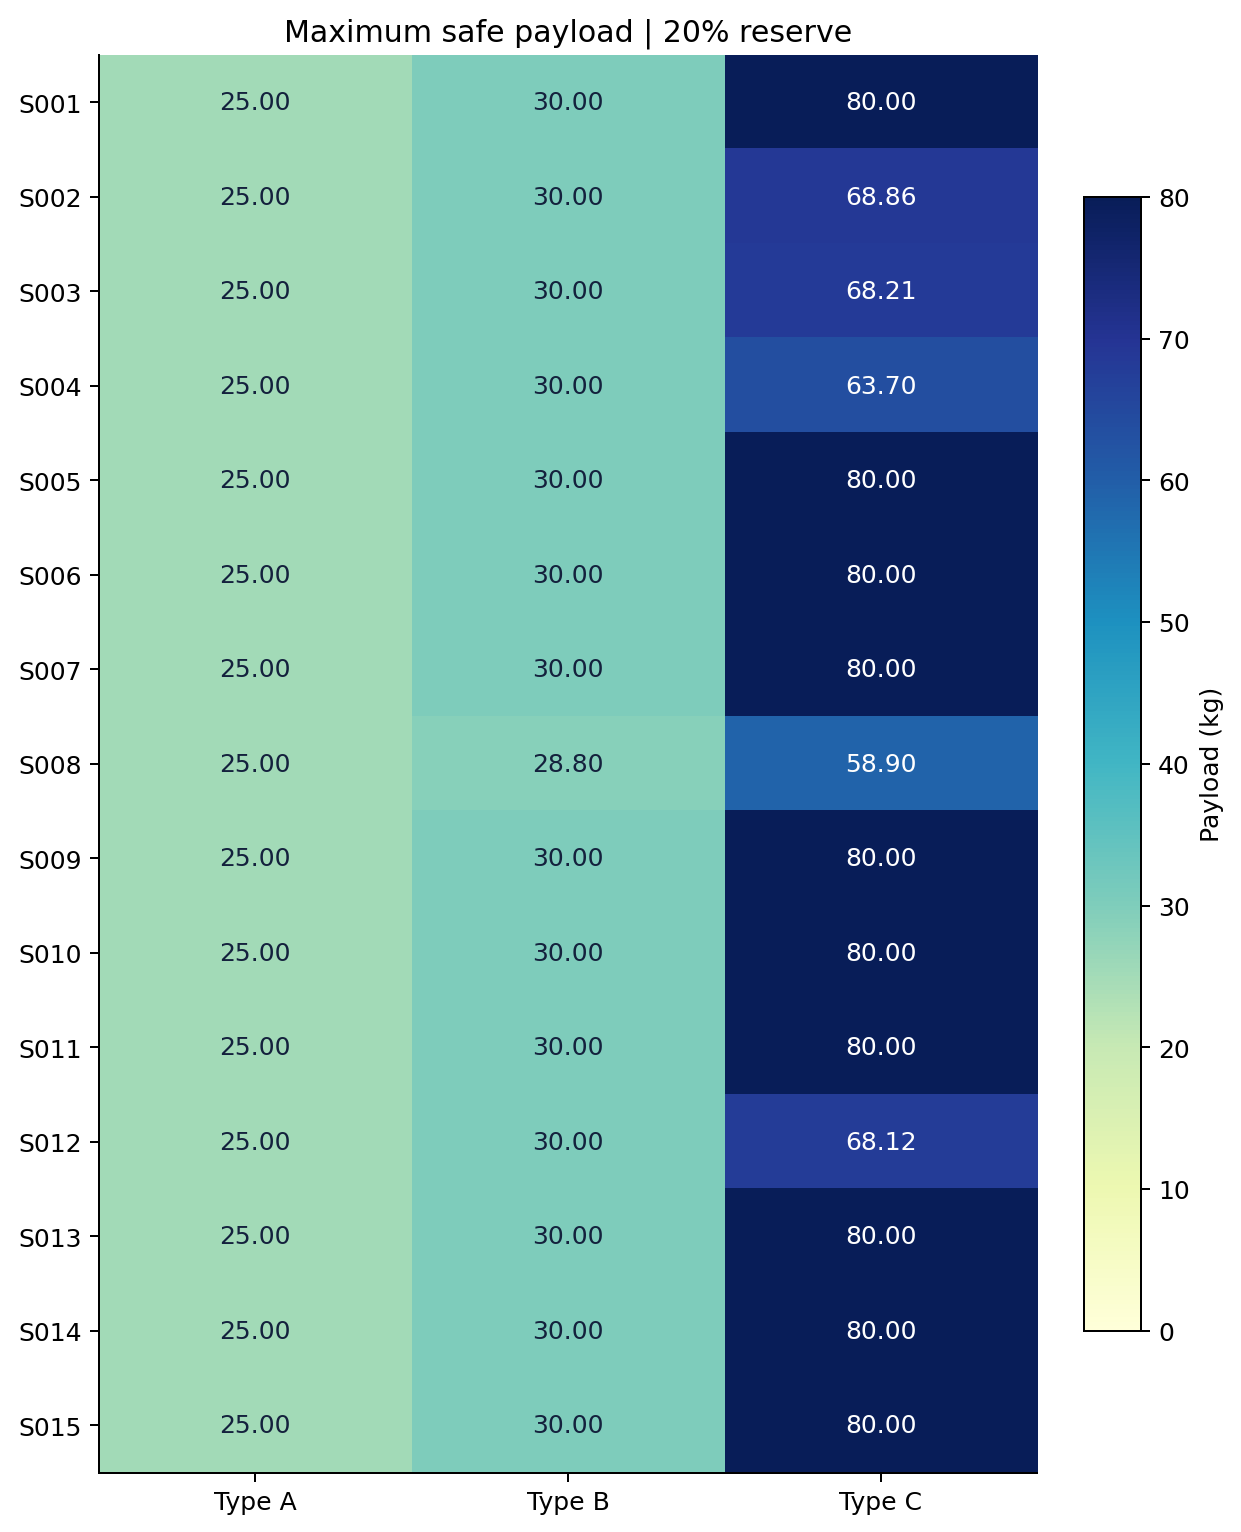
\includegraphics[width=0.74\textwidth]{safe_payload_heatmap.png}
  \caption{20\%返航安全余量下15个服务区与三类机型的最大安全载荷。}
  \label{fig:q1_safe_payload_heatmap}
\end{figure}

图\ref{fig:q1_safe_payload_heatmap}给出了全部45组结果。后续组批时，额定质量约束与能量约束仍分别计算；$w_{im}^{safe}$主要用于直观描述不同“机型--服务区”组合的运输能力边界。

\subsection{不可拆货箱组批优化模型}

\subsubsection{可行批型生成}

记服务区$i$的货箱集合为$\mathcal B_i$。对于任意非空货箱子集$S\subseteq\mathcal B_i$和机型$m$，若同时满足
\[
\sum_{b\in S}\mu_b\le Q_m,
\]
\[
\sum_{b\in S}\nu_b\le V_m,
\]
以及
\[
E_{im}\left(\sum_{b\in S}\mu_b\right)
\le(1-\alpha_m)E_m,
\]
则称$(i,m,S)$为一个\textbf{可行批型}。对每个批型$p$，预先计算其机型$m_p$、货箱集合$\mathcal B_p$、能耗$E_p$和完整作业时间$T_p$。

由于问题一禁止跨服务区组批，候选批型只在各服务区内部生成。这样既保留了原始货箱不可拆分约束，也将连续物理模型转换为有限的离散候选集合
\[
\mathcal P=\bigcup_{i\in\mathcal S}\mathcal P_i.
\]

\subsubsection{0--1精确组批模型}

对每个候选批型$p\in\mathcal P$定义二元决策变量
\[
y_p=
\begin{cases}
1,&\text{选择批型 }p,\\
0,&\text{否则}.
\end{cases}
\]
每个原始货箱必须且只能被配送一次，因此
\[
\sum_{p:b\in\mathcal B_p}y_p=1,
\qquad
\forall b\in\mathcal B.
\]

题目同时要求考虑架次数、总运输能耗和累计作业时间。为避免人为权重改变不同方案的排序，本文采用明确的词典序目标：
\[
\boxed{
\min_{\rm lex}
\left(
\sum_p y_p,\;
\sum_p E_py_p,\;
\sum_p T_py_p
\right).
}
\]
具体求解时分三层进行：第一层先求最少架次数$N^*$；第二层固定$N=N^*$后最小化总能耗；第三层再固定前两层最优值，最小化累计作业时间。这样可以使三项指标的比较顺序保持透明，并避免综合权重选择对结论产生额外影响。

\subsubsection{求解方法与交叉验证}

为保证组批结果不依赖单一求解器实现，本文采用三条精确求解路径进行交叉核验。

第一种是\textbf{原始箱级MILP}，直接保留原始货箱编号并对可行批型进行0--1选择；第二种是\textbf{对称压缩MILP}，将同一区域内属性完全相同的等价货箱进行计数压缩，减少由箱号置换产生的对称解；第三种是\textbf{剩余需求状态DP}，以各类货箱剩余数量为状态进行递推。

若状态记为
\[
\mathbf n=(n_1,n_2,\ldots,n_K),
\]
批型$p$对应的货箱计数向量为$\mathbf c_p$，则状态转移为
\[
\mathbf n\rightarrow\mathbf n-\mathbf c_p.
\]
在词典序求解中，DP只保留当前状态下更优的$(N,E,T)$标签；在Pareto分析中，则删除被其他标签同时支配的状态，保留非支配集合。

\begin{table}[H]
\centering
\caption{问题一三种精确求解方法及其作用}
\label{tab:q1_crosscheck}
\begin{tabular}{lll}
\toprule
方法 & 主要作用 & 核验结果\\
\midrule
原始箱级MILP & 保留原始箱号，直接求解0--1组批 & 与另外两种方法一致\\
对称压缩MILP & 消除等价货箱的箱号对称 & 与箱级MILP一致\\
剩余需求状态DP & 独立递推并生成Pareto标签 & 与MILP一致\\
\bottomrule
\end{tabular}
\end{table}

在20\%安全余量下，程序共生成742个满足容量条件的候选计数批型，经完整质量、体积与能量校验后保留732个可行批型。15个服务区的三种方法均得到相同的词典序目标。由此，后续正式方案不仅有一组可行解，还具有独立精确算法的一致性验证。

\subsection{模型求解与结果分析}

\subsubsection{最少架次数与最优性说明}

三类机型中最大额定载荷为80 kg。S001的总需求质量为154 kg，S002和S003均为81 kg，因此这三个服务区无论采用何种机型均至少需要2个架次；其余12个服务区至少需要1个架次。于是可得到全局架次数下界
\[
N\ge 2+2+2+12=18.
\]

精确组批模型找到了满足所有质量、体积和返航能量约束的18架次方案，因此
\[
\boxed{N^*=18}.
\]
在固定18架次后继续优化能耗和累计作业时间，得到
\[
\boxed{
E^*=59.131296\ {\rm kWh},
\qquad
T^{sum}=546.266929\ {\rm min}.
}
\]
最终机型构成为
\[
\boxed{A/B/C=0/9/9}.
\]

这里的“18架次最优”并不是因为求解器在搜索中没有找到更少方案，而是因为18同时具有可行上界和解析下界，二者闭合。

\subsubsection{各服务区正式运输方案}

为了使结果能够直接对应题目中的15个服务区，表\ref{tab:q1_area_plan}按服务区汇总18个正式架次。完整原始货箱编号及每个架次的体积、SOC等信息列于附录。

\scriptsize
\begin{longtable}{lccrrr}
\caption{问题一18架次正式方案的服务区汇总}\label{tab:q1_area_plan}\\
\toprule
服务区 & 架次数 & 机型构成 & 配送质量/kg & 能耗/kWh & 累计作业时间/min\\
\midrule
\endfirsthead
\toprule
服务区 & 架次数 & 机型构成 & 配送质量/kg & 能耗/kWh & 累计作业时间/min\\
\midrule
\endhead
S001 & 2 & C+C & 154 & 5.913351 & 53.106\\
S002 & 2 & B+C & 81 & 8.434647 & 64.308\\
S003 & 2 & B+C & 81 & 8.544882 & 74.177\\
S004 & 1 & C & 59 & 6.152932 & 38.351\\
S005 & 1 & C & 59 & 4.222193 & 31.287\\
S006 & 1 & C & 59 & 2.597988 & 26.026\\
S007 & 1 & C & 45 & 3.410894 & 31.793\\
S008 & 1 & C & 45 & 5.836012 & 36.662\\
S009 & 1 & B & 25 & 2.096234 & 25.974\\
S010 & 1 & B & 25 & 1.823196 & 25.923\\
S011 & 1 & B & 25 & 1.073952 & 19.807\\
S012 & 1 & B & 25 & 2.752414 & 32.046\\
S013 & 1 & B & 25 & 1.824759 & 25.175\\
S014 & 1 & B & 25 & 2.140388 & 31.163\\
S015 & 1 & B & 25 & 2.307453 & 30.471\\
\midrule
总计 & 18 & A/B/C=0/9/9 & 758 & 59.131296 & 546.267\\
\bottomrule
\end{longtable}
\normalsize

表\ref{tab:q1_area_plan}表明，架次数由各服务区不可跨区组批的规则和单架最大载荷共同决定；而在已经达到18架次以后，B、C两类机型的混合使用进一步降低了能耗与累计作业时间。S001、S002和S003均需要2个架次，其余服务区各1个架次，与前述下界结构完全一致。

\begin{figure}[H]
  \centering
  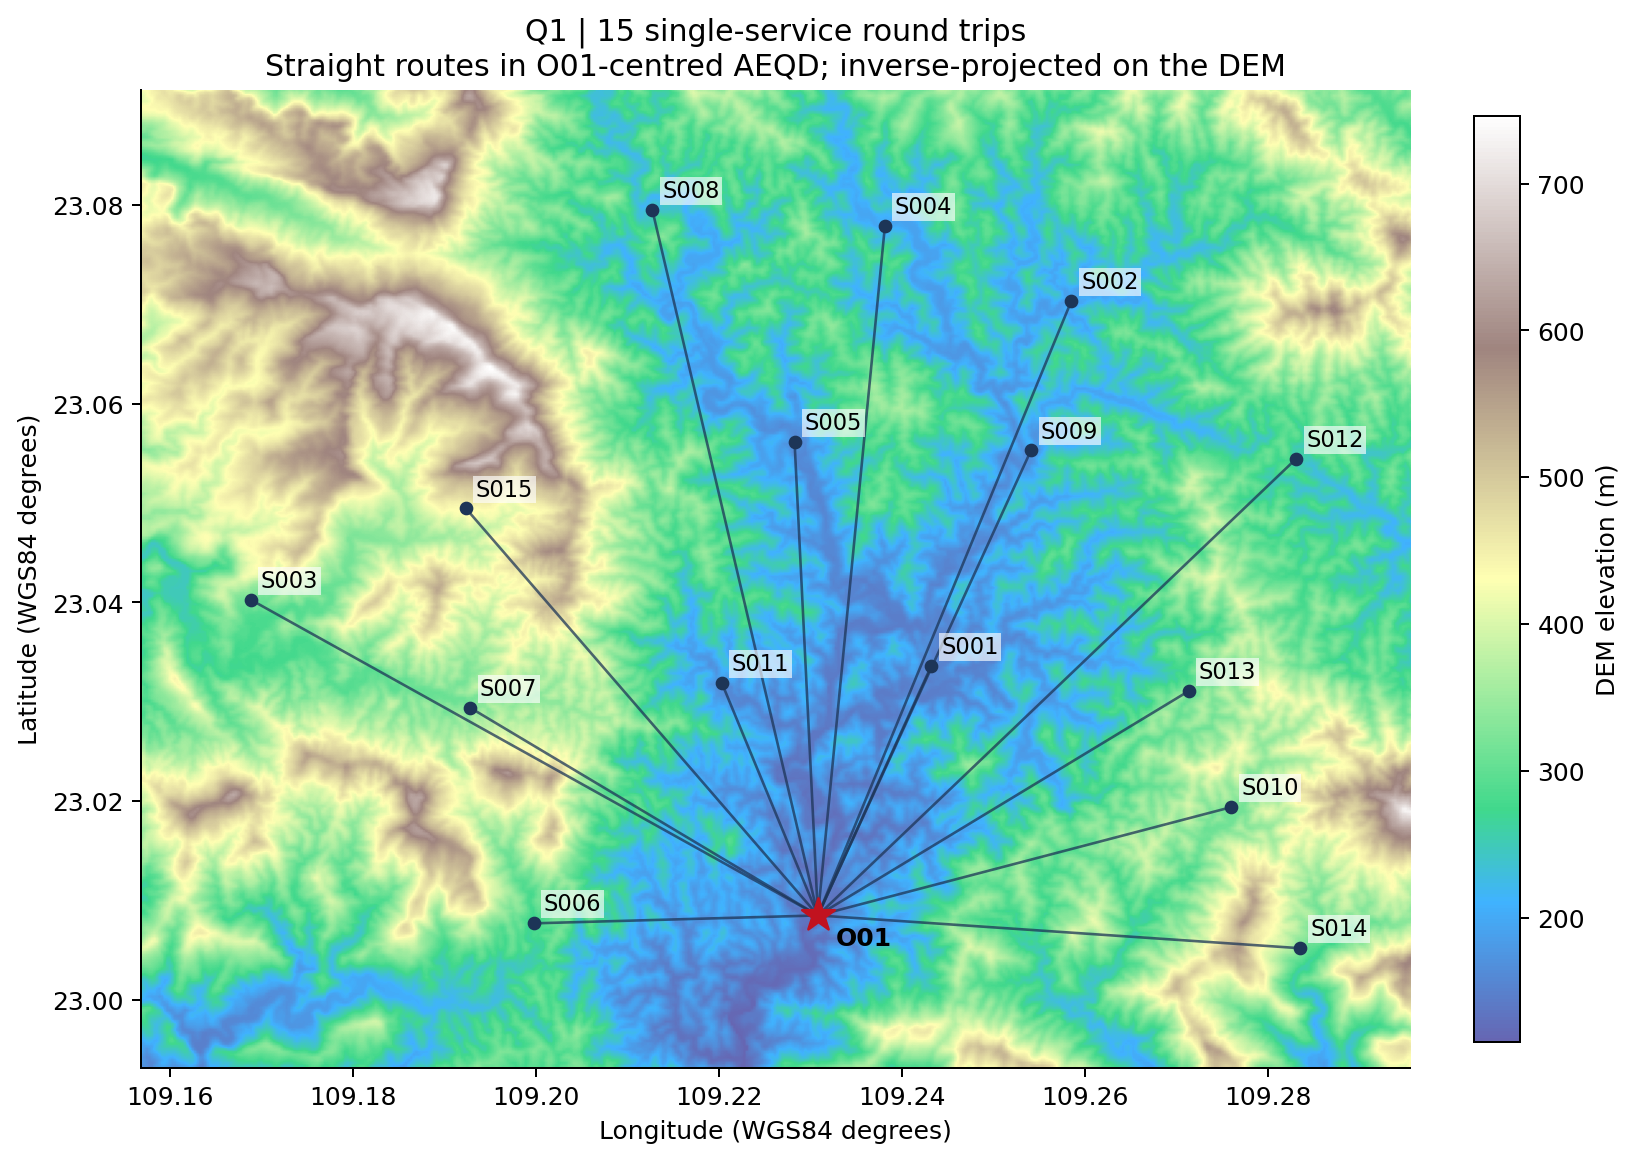
\includegraphics[width=0.82\textwidth]{map_single_routes.png}
  \caption{问题一基地O01至15个服务区的单点往返任务空间关系。每个架次均严格采用单服务区直接往返形式。}
  \label{fig:q1_single_routes}
\end{figure}

\subsubsection{基线比较与多目标权衡}

仅达到18架次并不能说明组批和机型选择已经充分优化。为此，将正式混合机型精确方案与单机型精确方案以及FFD质量优先基线进行比较，结果见表\ref{tab:q1_baseline_main}。

\begin{table}[H]
\centering
\caption{问题一主要基线与正式方案比较}
\label{tab:q1_baseline_main}
\begin{tabular}{llrrr}
\toprule
机型策略 & 方法 & 架次 & 能耗/kWh & 累计作业时间/min\\
\midrule
仅A型 & 精确 & 52 & 112.180153 & 1488.763007\\
仅B型 & 精确 & 35 & 68.350657 & 927.625473\\
仅C型 & 精确 & 18 & 73.934908 & 563.979235\\
混合机型 & FFD-质量 & 18 & 75.116697 & 563.979235\\
混合机型 & 精确 & \textbf{18} & \textbf{59.131296} & \textbf{546.266929}\\
\bottomrule
\end{tabular}
\end{table}

C型单机型精确方案已经能够达到18架次，但正式混合机型方案在架次数不变的条件下，相比仅C型精确方案进一步节省约20.02\%的能耗，并缩短17.712 min累计作业时间；相比混合机型FFD-质量基线，能耗下降约21.28\%。因此，本问的优化不能在“找到18架次”后停止，机型与箱组的联合选择仍具有明显价值。

对所有可行方案进行离散Pareto分析后，最终不同的非支配目标向量只有两组：
\[
(18,\ 59.131296,\ 546.266929),
\]
\[
(19,\ 59.033942,\ 573.999623),
\]
其中三元组依次表示“架次数、总能耗、累计作业时间”。从18架次增加到19架次仅节省约0.097354 kWh，即约0.165\%能耗，却使累计作业时间增加约27.733 min。因此，在题目强调架次数优先的条件下，18架次方案具有更合理的综合表现。

\begin{figure}[H]
  \centering
  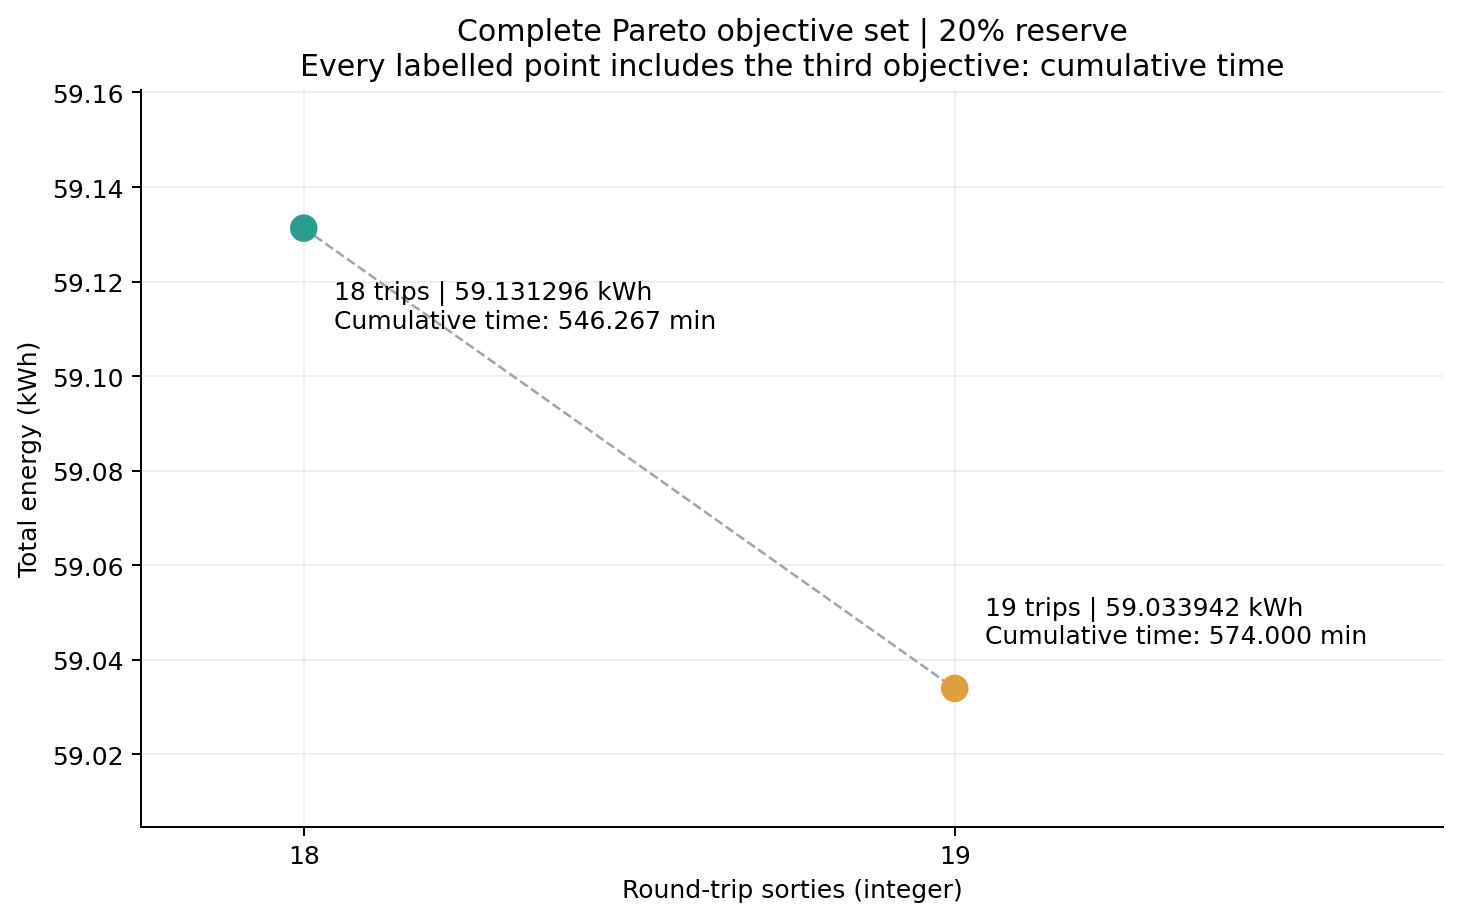
\includegraphics[width=0.78\textwidth]{pareto_front.png}
  \caption{问题一完整离散Pareto目标集合。19架次方案仅换取极小能耗下降，却显著增加累计作业时间。}
  \label{fig:q1_pareto}
\end{figure}

\subsection{返航安全余量敏感性分析}

\subsubsection{安全余量对载荷能力的影响}

基准模型采用20\%返航安全余量。为分析安全要求变化对运输能力的影响，对所有候选批型定义
\[
\rho_p=1-\frac{E_p}{E_{m_p}},
\]
则在统一安全余量$\alpha$下，批型$p$可行当且仅当
\[
\alpha\le\rho_p.
\]
随着$\alpha$增加，可使用的能源预算$(1-\alpha)E_m$连续下降，相应最大安全载荷也随之下降。

\begin{figure}[H]
  \centering
  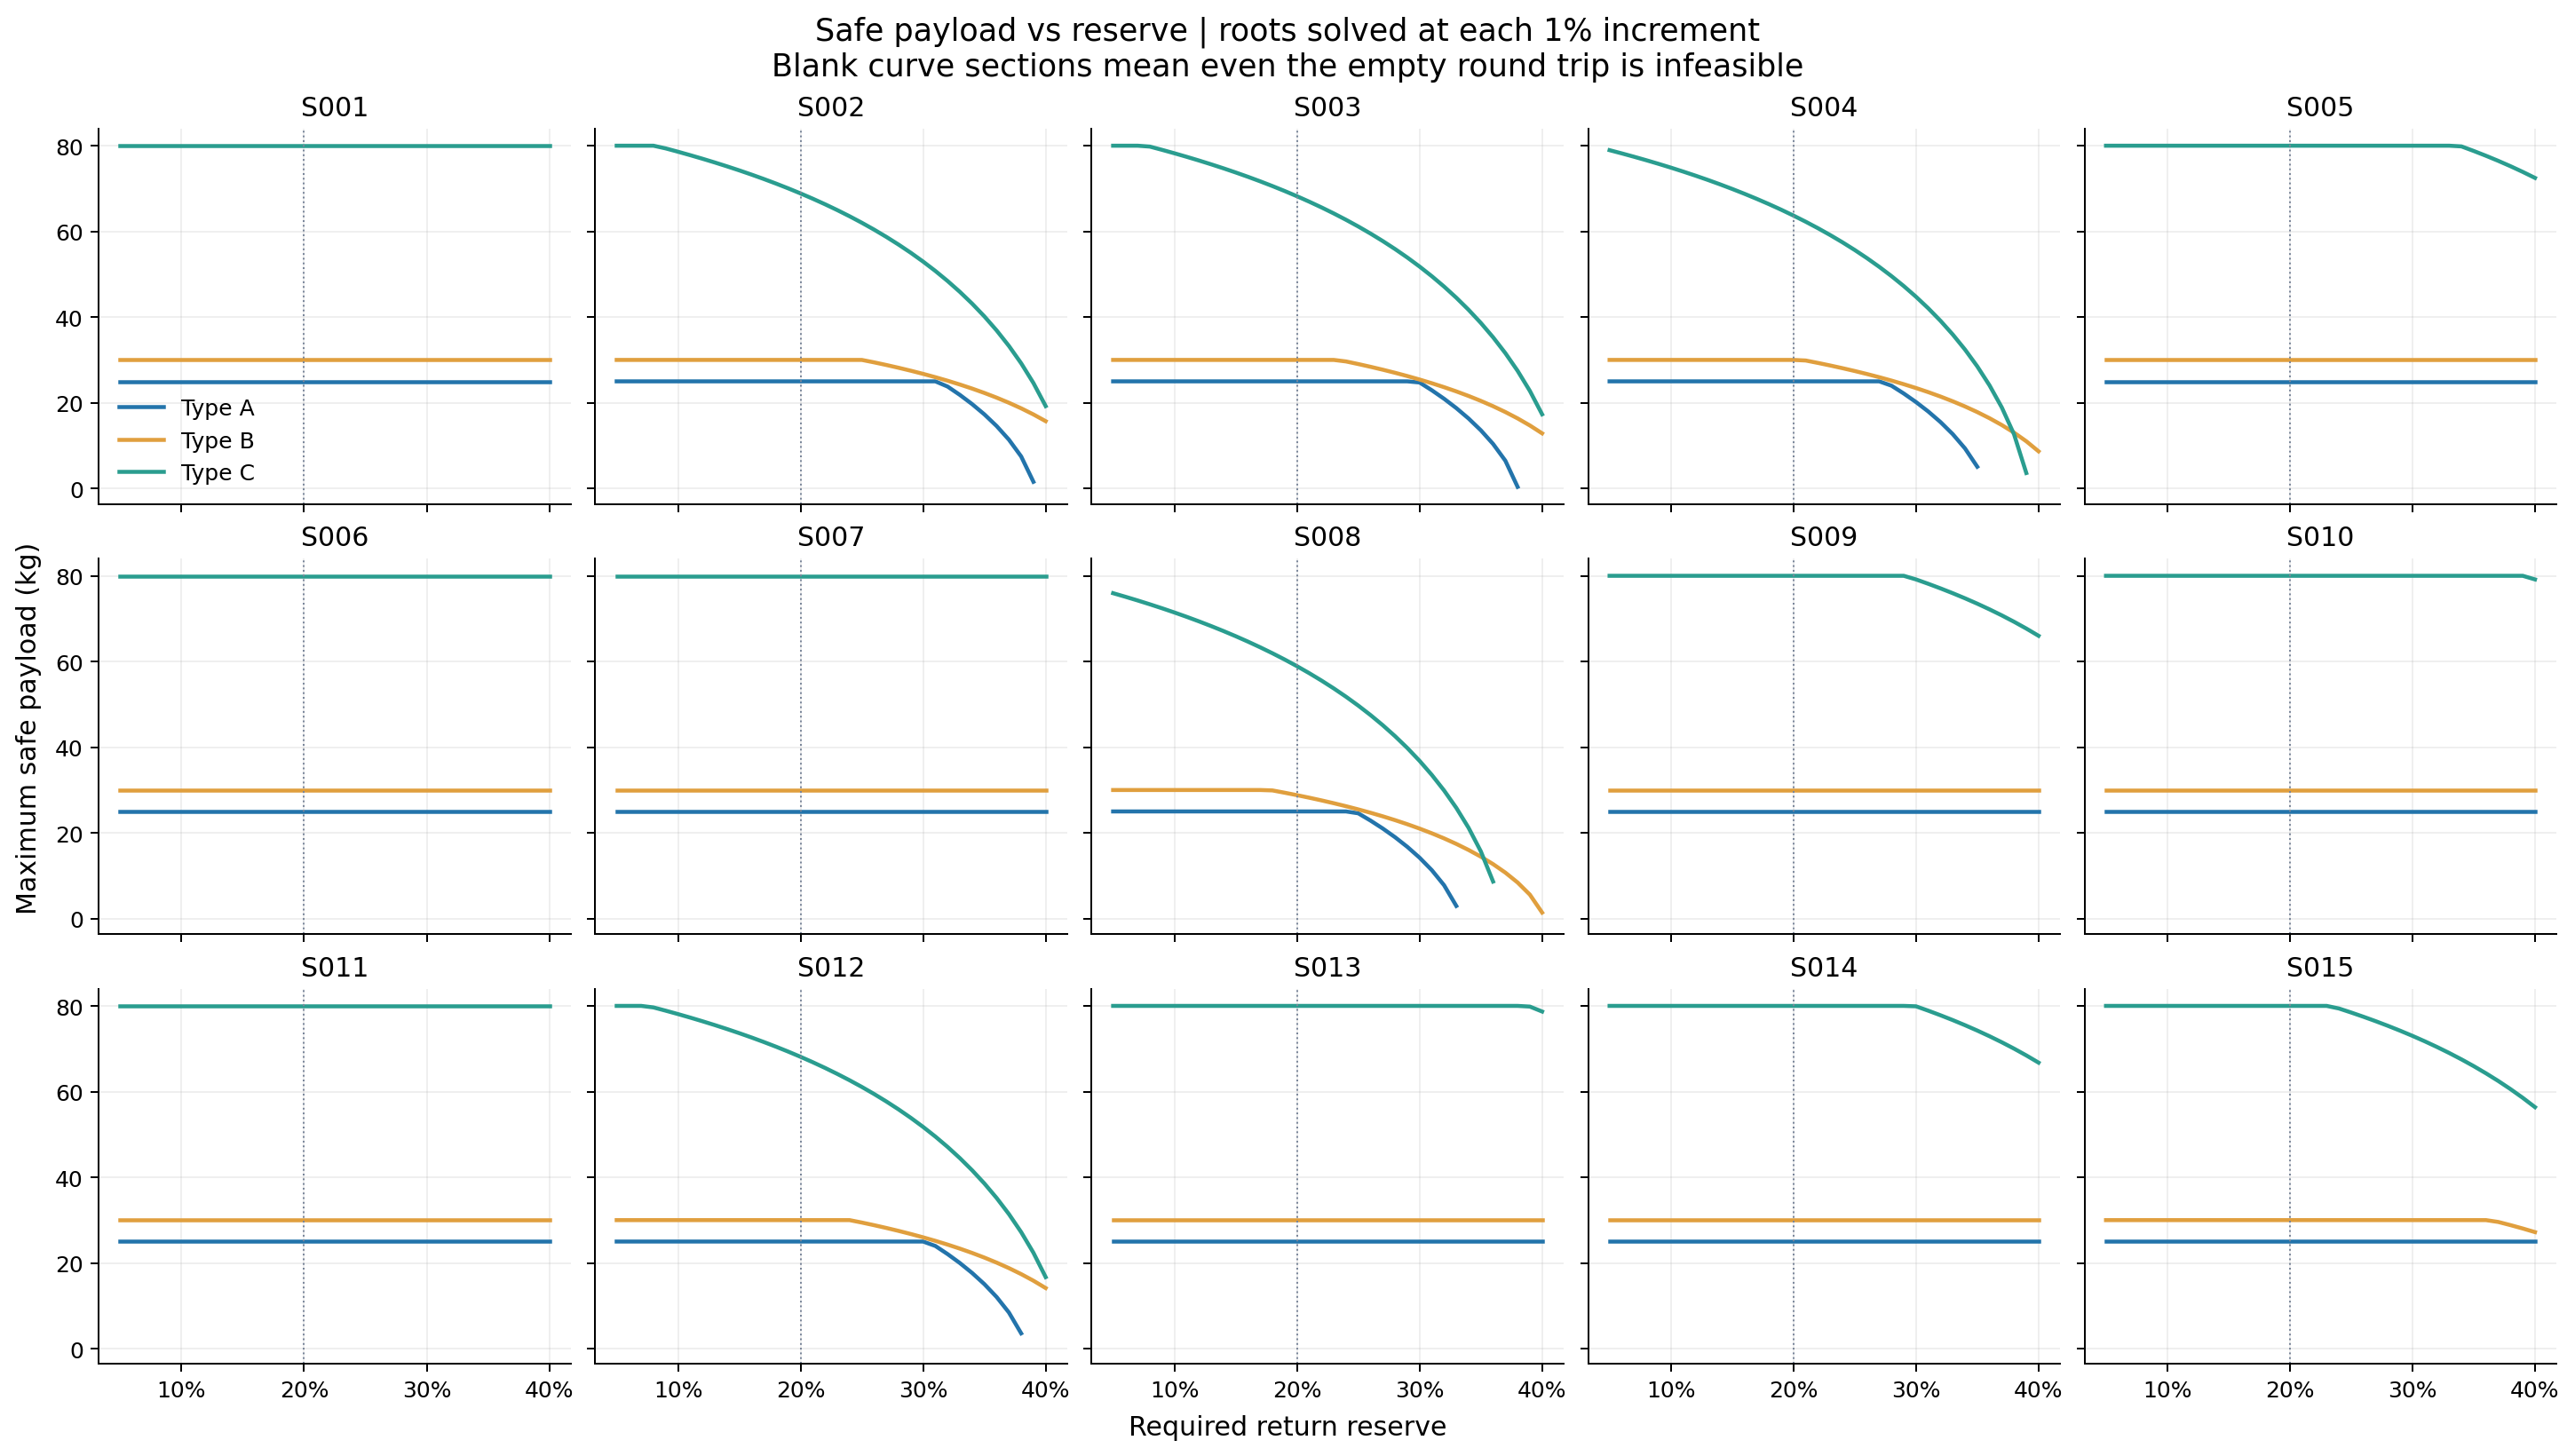
\includegraphics[width=0.96\textwidth]{reserve_vs_safe_payload.png}
  \caption{返航安全余量变化下各服务区三类机型最大安全载荷的变化。}
  \label{fig:q1_reserve_payload}
\end{figure}

\subsubsection{连续安全参数引起的离散架次跃迁}

货箱不可拆分使系统响应并非连续变化。完整计算共得到569个候选安全余量事件，其中只有8个事件真正改变全局最少架次数，如表\ref{tab:q1_reserve_events}所示。

\begin{table}[H]
\centering
\caption{改变全局最少架次数的8个安全余量临界事件}
\label{tab:q1_reserve_events}
\begin{tabular}{lcrr}
\toprule
临界余量/\% & 触发服务区 & 阈值处架次 & 严格右侧架次\\
\midrule
23.088350 & S004 & 18 & 19\\
27.049854 & S008 & 19 & 20\\
33.625809 & S008 & 20 & 21\\
33.896918 & S003 & 21 & 22\\
34.373532 & S004 & 22 & 23\\
34.391873 & S002 & 23 & 24\\
34.777897 & S008 & 24 & 25\\
35.267807 & S008 & 25 & 不可行\\
\bottomrule
\end{tabular}
\end{table}

当安全余量由20\%提高到23.08835\%以内时，最少架次数仍保持18；一旦严格超过该阈值，S004原有关键批型失效，最少架次数增至19。继续提高安全余量后，架次数在若干离散阈值处逐级增加。当$\alpha>35.267807\%$时，S008的一只14 kg饮用水箱即使单独运输，也不能由任一机型完成满足返航余量的往返任务，因此整个问题失去可行解。

\begin{figure}[H]
  \centering
  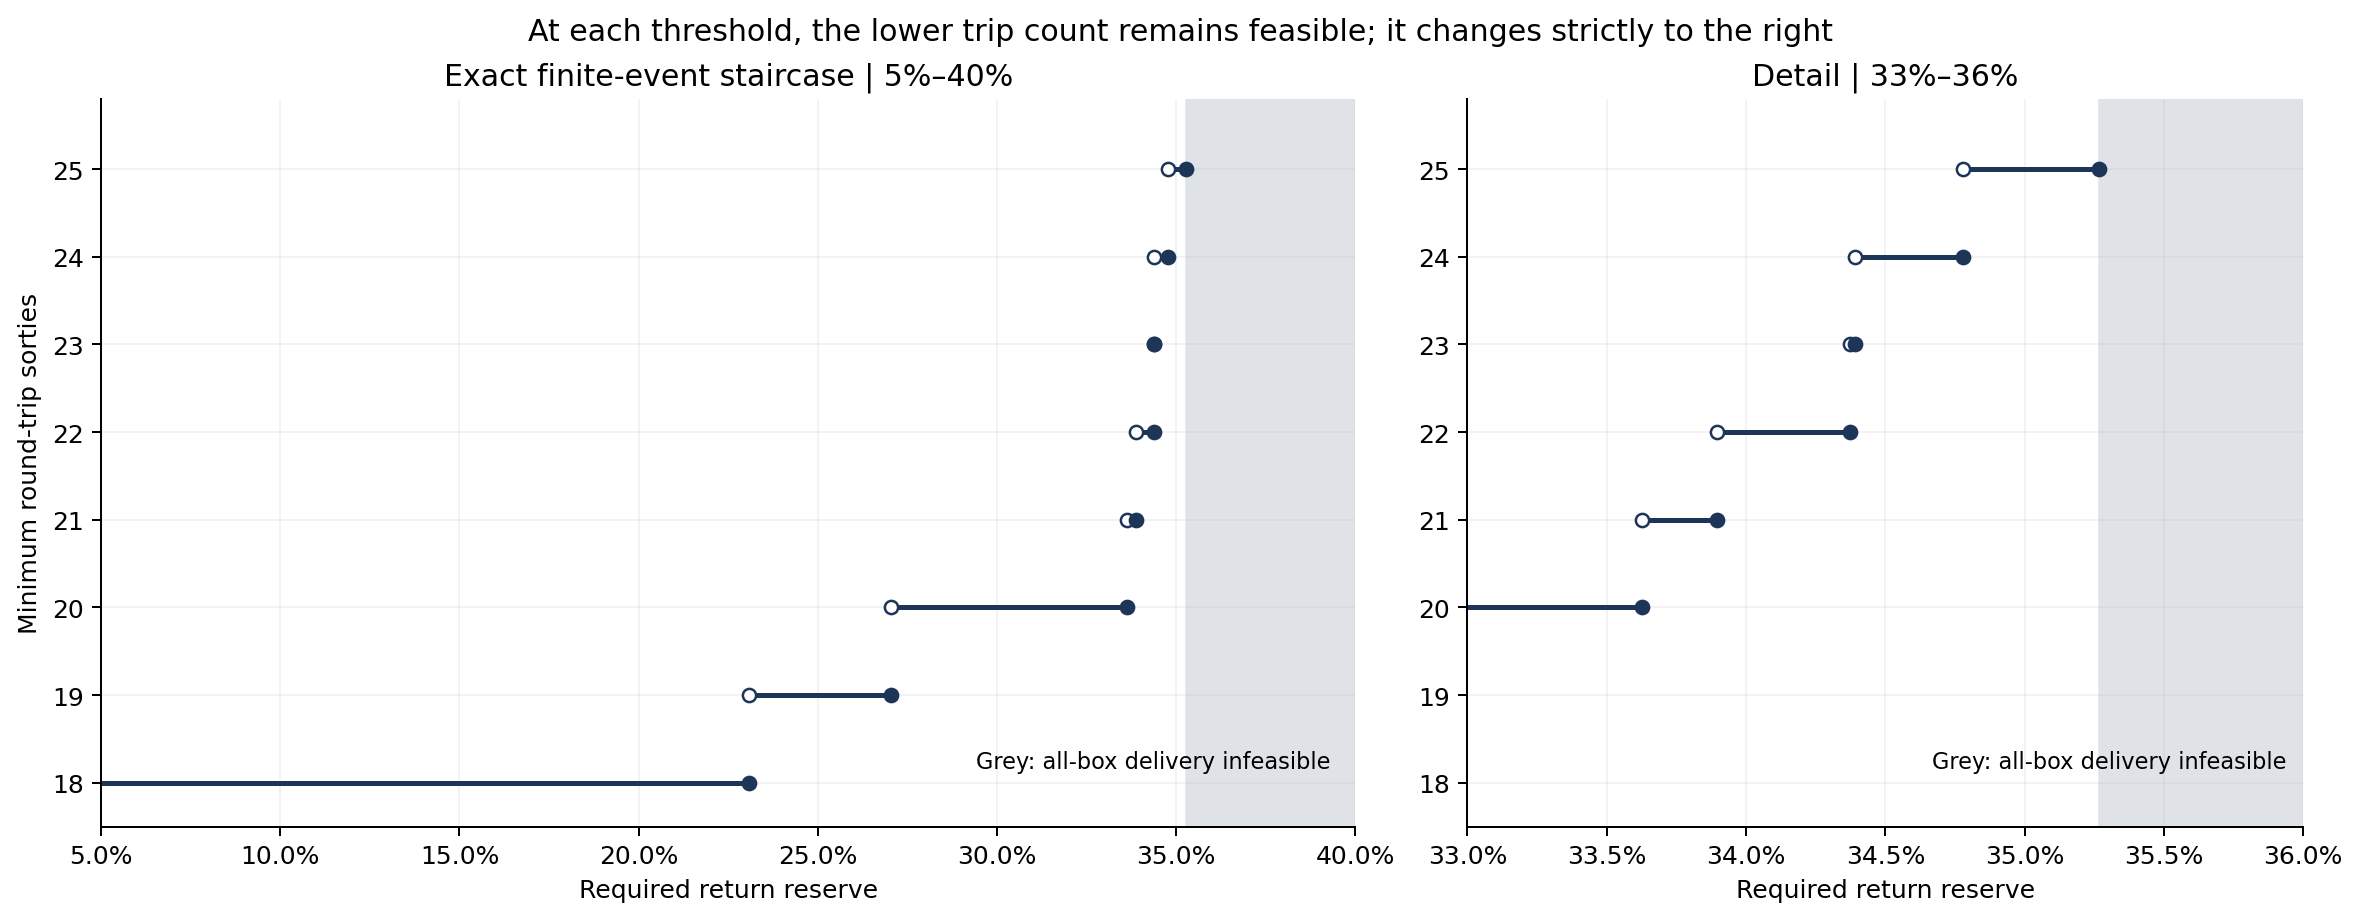
\includegraphics[width=0.95\textwidth]{reserve_vs_min_sorties.png}
  \caption{返航安全余量变化引起的最少架次数阶梯跃迁。连续的安全要求通过不可拆货箱约束转化为离散决策变化。}
  \label{fig:q1_reserve_sorties}
\end{figure}

由此可以得到问题一的核心结论：在20\%返航安全余量下，18架次为可证明的最少运输架次数；在该架次数上，混合使用B、C型无人机可将总能耗降至59.131296 kWh、累计作业时间降至546.266929 min。与此同时，安全余量不是一个只影响“剩余电量”的连续参数，它会通过不可拆组批结构在若干临界点直接改变所需架次数甚至使任务失去可行性。


\clearpage
\section{问题二：异构多架次运输与共享电池联合调度}
\label{sec:q2}

\subsection{问题分析}

问题一解决的是“单个架次能否安全完成”和“同一服务区内部如何组批”，而问题二进一步要求在真实有限资源条件下完成全部80个货箱的配送。此时，一项运输任务即使在质量、体积和能量上完全可行，也可能因为实体无人机尚未返航、共享电池仍在充电或关键货箱送达过晚而无法进入完整时间表。因此，本问的核心已经由单架次组批优化转变为
\[
\boxed{
\text{货箱组批}
+
\text{多点访问}
+
\text{机型选择}
+
\text{飞机--电池双资源排程}
+
\text{箱级时限}
}
\]
共同作用的异构联合调度问题。

与问题一相比，本问增加了三类关键耦合关系。

第一，\textbf{组批与路线耦合}。一个运输架次可以访问多个服务区，访问顺序不仅改变飞行距离，还改变逐段剩余载荷、能耗和每个货箱的实际送达时刻。

第二，\textbf{任务与双资源耦合}。每个架次必须同时占用一架兼容的实体无人机和一组对应型号的满电电池。无人机返航后可以立即释放，但电池仍需经历充电恢复，因此
\[
\boxed{
\text{无人机返航}
\neq
\text{电池重新可用}.
}
\]

第三，\textbf{局部任务与系统工期耦合}。减少单个架次时间或架次数，并不一定缩短整个机群最后返航时间；真正决定系统完成时间的是各机型资源链上的关键任务及其电池恢复时刻。

因此，本问不能先生成若干运输任务再独立“排一张时间表”，而应在任务结构、路线和资源时序之间反复调整，直到形成完整可执行方案。

\subsection{求解思路与总体框架}

结合题目要求和上述耦合关系，本文采用“\textbf{可行方案搜索 + 独立质量认证}”的双路线求解框架。可行方案路线负责寻找真实可执行的高质量运输计划，认证路线则在不改变正式方案的前提下给出完成时间的全局有效下界。

\begin{figure}[H]
  \centering
  \resizebox{0.94\textwidth}{!}{\QTwoFigFramework}
  \caption{问题二总体求解框架。左侧构造并改进真实可执行调度方案，右侧独立计算全局有效下界，最终形成可核验的完成时间区间。}
  \label{fig:q2_framework_v7}
\end{figure}

具体求解分为五个步骤。

\begin{enumerate}[label=\textbf{步骤\arabic*.},leftmargin=4.5em]
  \item 由第3章公共物理模型生成运输任务表示，计算每个候选任务的路线、作业时长、能耗、返航SOC和逐箱送达偏移；
  \item 建立货箱覆盖、机型兼容、实体飞机、共享电池、充电恢复和箱级时限组成的联合调度模型；
  \item 使用飞机--电池事件解码器将任务序列还原为真实资源时间表，并对全部80个货箱进行逐箱时限检查；
  \item 采用自适应大邻域搜索对货箱分配、访问路线、机型和任务顺序进行破坏--修复与局部强化，持续改善可行上界；
  \item 对正式方案进行独立重放，并通过固定任务瓶颈、22架次对照和全局有效下界分析评价方案质量。
\end{enumerate}

该流程与优秀竞赛论文常用的“问题分解--模型建立--算法求解--方案输出--结果验证”结构一致：模型负责说明什么方案才是可行的，算法负责说明如何在巨大组合空间中找到方案，结果部分则必须给出具体的运输与资源安排，而不是只报告总工期。

\subsection{异构多架次联合调度模型建立}

\subsubsection{运输任务表示与决策变量}

设搜索过程中由货箱集合、机型和访问顺序构成的物理可行运输任务集合为$\mathcal C$。对任务$r\in\mathcal C$，第3章公共模型已经给出
\[
r=(m_r,\mathcal B_r,\pi_r,p_r,E_r,SOC_r^{return},\{\delta_{rb}\}),
\]
其中$m_r$为机型，$\mathcal B_r$为携带货箱集合，$\pi_r$为有序访问路线，$p_r$为完整作业时长，$E_r$为能耗，$\delta_{rb}$为货箱$b$相对任务开始的送达偏移。

定义
\[
x_r=
\begin{cases}
1,&\text{选择任务 }r,\\
0,&\text{否则},
\end{cases}
\]
并令$a_{ru}$表示任务$r$是否由实体无人机$u$执行，$b_{rk}$表示是否使用共享电池$k$，$s_r$为任务开始时刻。

每个原始货箱必须且只能被某一个已选任务配送：
\[
\boxed{
\sum_{r\in\mathcal C:b\in\mathcal B_r}x_r=1,
\qquad \forall b\in\mathcal B.
}
\]
每个被选择任务必须分配给唯一兼容实体无人机和唯一兼容电池：
\[
\sum_{u\in\mathcal U_{m_r}}a_{ru}=x_r,
\qquad
\sum_{k\in\mathcal K_{m_r}}b_{rk}=x_r.
\]

候选任务本身已经通过第3章的质量、体积、路线和返航安全能量检查，因此这些物理约束不在本节重复展开。

\subsubsection{飞机--电池双资源占用约束}

若任务$r$在$s_r$开始，实体无人机从准备阶段开始占用，直至任务返航，其占用区间为
\[
I_r^U=[s_r,s_r+p_r).
\]
设返航后的充电恢复时间为
\[
c_r=\tau(SOC_r^{return}),
\]
其中$\tau(\cdot)$为第3章给出的两阶段充电函数，则对应电池的占用区间为
\[
I_r^B=[s_r,s_r+p_r+c_r).
\]
同一实体无人机不能同时执行两个任务，同一电池也不能在充电完成前再次投入使用，因此
\[
a_{ru}=a_{r'u}=1
\Longrightarrow
I_r^U\cap I_{r'}^U=\varnothing,
\]
\[
b_{rk}=b_{r'k}=1
\Longrightarrow
I_r^B\cap I_{r'}^B=\varnothing.
\]

\begin{figure}[H]
  \centering
  \resizebox{0.86\textwidth}{!}{\QTwoFigOccupancy}
  \caption{单个运输任务对实体无人机和共享电池的不同占用区间。返航只释放飞机资源，原电池仍需充电至100\%后才能再次使用。}
  \label{fig:q2_resource_occupancy_v7}
\end{figure}

该约束是问题二区别于普通车辆路径问题的重要之处：飞机和电池属于两个可以分离、但必须在任务开始时同时可用的资源池。

\subsubsection{箱级送达时限约束}

若货箱$b$由任务$r$运输，则其实际送达时刻为
\[
C_b=s_r+\delta_{rb}.
\]
对于医疗物资和题目指定的首批保障货箱，按照对应硬性时间要求必须满足
\[
C_b\le h_b.
\]
对于其余货箱，记期望送达时间为$d_b$，定义迟到量
\[
L_b=\max(0,C_b-d_b),
\]
并按照货箱优先级$\omega_b$计算加权迟到
\[
L_w=\sum_{b\in\mathcal B}\omega_bL_b.
\]
硬截止属于可行性约束，不能通过降低能耗或减少架次数进行补偿。

\subsubsection{优化目标}

题目同时要求考虑配送及时性、全部任务完成时间、能耗和架次数。为避免人为权重使不同量纲指标相互抵消，本文采用词典序评价：
\[
\boxed{
\min_{\rm lex}(L_w,T_{\max},E,N)
}
\]
其中
\[
T_{\max}=\max_{r:x_r=1}(s_r+p_r),
\qquad
E=\sum_rx_rE_r,
\qquad
N=\sum_rx_r.
\]

即首先尽可能保证所有货箱按期送达；在相同及时性水平下，优先缩短所有运输无人机最后返航时间；再比较总能耗和架次数。正式方案达到$L_w=0$，由于$L_w\ge0$，因此第一层目标已经达到全局最优值0。

\subsection{模型求解算法设计}

\subsubsection{任务编码与飞机--电池事件解码}

完整模型同时包含货箱组批、路线排列、机型和资源时间安排，直接枚举全部组合不可行。实际求解将一个候选方案编码为运输任务序列
\[
S=(r_1,r_2,\ldots,r_N).
\]
每个任务保存机型、原始货箱集合和访问顺序。任何任务被修改后，都重新调用统一物理评价器计算逐段载荷、飞行时间、能耗、返航SOC、充电时间和逐箱送达偏移，避免启发式搜索使用近似物理量。

对每种机型分别维护实体无人机与电池的最早可用时刻。若当前任务$r$所选最早可用飞机时刻为$t_u$、最早可用电池时刻为$t_k$，则
\[
\boxed{
s_r=\max(t_u,t_k).
}
\]
任务结束后更新
\[
t_u\leftarrow s_r+p_r,
\qquad
t_k\leftarrow s_r+p_r+\tau(SOC_r^{return}).
\]
完成全部任务解码后，再逐箱检查硬截止、加权迟到和送达时刻。由此，一个“看起来装得下”的任务组合只有经过完整飞机--电池事件重放后，才可能成为正式可行方案。

\subsubsection{自适应大邻域搜索}

可行上界搜索采用自适应大邻域搜索（ALNS）思想。每轮从当前方案中破坏一部分任务结构，再重新修复并进行局部强化。实际实现包含四类破坏算子：

\begin{itemize}
  \item \textbf{随机破坏}：随机移除3--7个货箱；
  \item \textbf{路线破坏}：移除一条或少量完整运输任务中的货箱；
  \item \textbf{相关破坏}：优先移除空间位置接近的服务区货箱；
  \item \textbf{关键链破坏}：优先处理负载最高机型或工期关键任务。
\end{itemize}

修复阶段使用greedy、regret-2和regret-3三种插入策略。每个被移除货箱重新插入时，不只尝试原任务，还允许重新选择机型、访问顺序和任务位置；候选方案必须通过完整物理评价和事件解码。

局部强化进一步执行同型任务换序、任务改型、跨任务换箱和单箱迁移。搜索过程中使用标量代理分数提高探索效率，并采用随迭代衰减的接受概率跳出局部最优；但正式方案的最终比较始终使用前述词典序目标，搜索代理分数不作为论文最终评价指标。

破坏和修复算子的选择概率根据历史改进效果每25轮自适应更新，使搜索资源逐步集中到当前实例中更有效的邻域操作。

\begin{table}[H]
\centering
\caption{问题二自适应大邻域搜索主流程}
\label{tab:q2_alns_steps}
\begin{tabularx}{0.96\textwidth}{cX}
\toprule
步骤 & 操作\\
\midrule
1 & 读取当前可行任务序列，使用事件解码器生成飞机--电池时间表并计算正式指标。\\
2 & 按自适应权重选择随机、路线、相关或关键链破坏算子，移除部分货箱。\\
3 & 采用greedy、regret-2或regret-3策略重新插入，并重新选择可行机型与访问顺序。\\
4 & 对候选方案完整重算物理量并执行飞机、电池、充电和箱级时限重放。\\
5 & 进行任务换序、改型、换箱和单箱迁移等局部强化。\\
6 & 根据搜索代理分数与温度接受准则决定是否更新当前解；若词典序严格改善则更新最优解。\\
7 & 周期性更新破坏/修复算子权重，达到迭代或时间条件后输出最优可行方案。\\
\bottomrule
\end{tabularx}
\end{table}

\begin{figure}[H]
  \centering
  \resizebox{0.86\textwidth}{!}{\QTwoFigUpperSearch}
  \caption{问题二可行上界搜索与资源重放闭环。任务重构后的每个候选方案都必须重新通过真实飞机、电池、充电恢复和箱级时限检查。}
  \label{fig:q2_upper_search_v7}
\end{figure}

\subsubsection{独立验证}

正式解输出后，再使用与主求解器独立的验证程序重新读取原始节点、机型、货箱和航段数据，从零重建每个架次的载荷、飞行阶段、能耗、SOC、充电时间和送达时刻，并检查同一飞机/电池占用区间是否重叠。独立验证不调用主评价器的中间结果，从而降低“同一程序重复验证自身”的风险。

\subsection{模型求解与结果分析}

\subsubsection{正式23架次方案总体结果}

最终得到一组零加权迟到的23架次运输方案，机型构成为
\[
A/B/C=11/6/6.
\]
8架实体运输无人机全部投入任务，实际使用14组共享电池。系统最后返航时间为
\[
\boxed{
T_{\max}=5693.231489\ {\rm s}
=94.887191\ {\rm min},
}
\]
总运输能耗为
\[
\boxed{
E=66.214460\ {\rm kWh}.
}
\]

\begin{table}[H]
\centering
\caption{问题二正式主方案关键指标}
\label{tab:q2_main_metrics}
\begin{tabular}{lr}
\toprule
指标 & 结果\\
\midrule
货箱总数 & 80\\
加权迟到 & 0\\
硬迟到箱数 & 0\\
运输架次 & 23\\
A/B/C架次 & 11/6/6\\
实体运输无人机 & 8\\
实际使用共享电池 & 14\\
最后一箱送达时刻/s & 5283.168387\\
最后返航时间/s & 5693.231489\\
总运输能耗/kWh & 66.214460\\
最紧硬截止余量/s & 202.096058\\
最低返航SOC & 20.097383\%\\
\bottomrule
\end{tabular}
\end{table}

最后一箱在约88.053 min完成交付，而系统工期为94.887 min，二者相差约6.834 min。这说明题目定义的“全部任务完成时间”必须以最后一架无人机返航为准，不能用最后一个货箱的交付时刻替代。

\subsubsection{23架次飞机--电池调度表}

为使正式结果能够直接核验，表\ref{tab:q2_schedule_main}按照实际调度记录列出23个架次的机型、访问路线、实体无人机、共享电池以及开始/返航时间。货箱原始ID的完整分配列于附录。

\scriptsize
\begin{longtable}{lcp{3.1cm}ccrr}
\caption{问题二正式23架次的飞机--电池调度方案}\label{tab:q2_schedule_main}\\
\toprule
记录 & 机型 & 访问路线 & 飞机 & 电池 & 开始/min & 返航/min\\
\midrule
\endfirsthead
\toprule
记录 & 机型 & 访问路线 & 飞机 & 电池 & 开始/min & 返航/min\\
\midrule
\endhead
V5-01 & A & S007 & U01 & A-BAT01 & 0.00 & 28.79\\
V5-02 & A & S015 & U02 & A-BAT02 & 0.00 & 32.81\\
V5-03 & A & S001 & U03 & A-BAT03 & 0.00 & 20.85\\
V5-04 & A & S009$\to$S002$\to$S013 & U04 & A-BAT04 & 0.00 & 44.59\\
V5-05 & B & S010 & U05 & B-BAT01 & 0.00 & 25.92\\
V5-06 & B & S004 & U06 & B-BAT02 & 0.00 & 32.03\\
V5-07 & C & S001 & U07 & C-BAT01 & 0.00 & 27.10\\
V5-08 & C & S001 & U08 & C-BAT02 & 0.00 & 23.80\\
V5-09 & A & S013 & U03 & A-BAT05 & 20.85 & 47.72\\
V5-10 & C & S006 & U08 & C-BAT03 & 23.80 & 49.83\\
V5-11 & B & S012 & U05 & B-BAT03 & 25.92 & 57.97\\
V5-12 & C & S002 & U07 & C-BAT04 & 27.10 & 63.33\\
V5-13 & A & S011$\to$S004 & U01 & A-BAT06 & 28.79 & 69.86\\
V5-14 & B & S014 & U06 & B-BAT04 & 32.03 & 63.19\\
V5-15 & A & S007 & U02 & A-BAT03 & 35.36 & 64.15\\
V5-16 & A & S003$\to$S015 & U04 & A-BAT01 & 46.61 & 90.00\\
V5-17 & C & S007$\to$S003 & U08 & C-BAT02 & 49.83 & 94.72\\
V5-18 & A & S004 & U03 & A-BAT02 & 53.46 & 89.77\\
V5-19 & B & S008 & U05 & B-BAT01 & 57.97 & 90.67\\
V5-20 & B & S008 & U06 & B-BAT02 & 63.19 & 94.89\\
V5-21 & C & S005 & U07 & C-BAT01 & 63.33 & 94.62\\
V5-22 & A & S009 & U02 & A-BAT05 & 65.80 & 93.95\\
V5-23 & A & S011 & U01 & A-BAT04 & 69.86 & 90.23\\
\bottomrule
\end{longtable}
\normalsize

从时间表可以看到，前8个架次在$t=0$并行启动，随后不同机型按照各自飞机和电池的释放时刻继续执行。特别是U06执行的V5-20在94.887 min返航，构成当前方案的系统工期端点。

\subsubsection{空间路线与资源时序}

\begin{figure}[H]
  \centering
  \resizebox{0.84\textwidth}{!}{\QTwoFigRouteMap}
  \caption{问题二正式23架次方案的空间路线与机型结构。多点任务主要用于在时限允许的条件下提高单架次利用率。}
  \label{fig:q2_route_map_v7}
\end{figure}

\begin{figure}[H]
  \centering
  \resizebox{0.98\textwidth}{!}{\QTwoFigGantt}
  \caption{问题二正式方案的飞机--电池双资源甘特图。上图给出8架实体运输无人机任务链，下图给出14组共享电池的任务占用与充电恢复。}
  \label{fig:q2_gantt_v7}
\end{figure}

空间路线图回答“每个架次飞到哪里”，调度表和甘特图回答“何时由哪架飞机、哪组电池执行”。三者结合后，正式方案能够同时对应题目要求的运输路线、架次安排、资源使用和系统完成时间。

\subsubsection{时限与资源可行性分析}

正式方案中80个货箱均恰好配送一次，医疗物资和首批保障货箱全部满足硬性时间要求，其他货箱加权迟到同样为0。最紧硬截止余量仍有202.096 s，说明零迟到并非由数值舍入得到。

返航SOC最低值为20.097383\%，略高于20\%安全余量下限，出现在当前高负载C型任务上。独立验证还检查了飞机占用区间和电池占用--充电区间，未发现任何同一资源重叠。因此该方案不仅在目标函数上表现良好，而且具有完整的资源可执行性。

\subsubsection{相对原方案的节能调整}

在保持23架次、零迟到和5693.231489 s工期不变的条件下，对S001两项C型同路线任务交换一只食品箱和一只卫生用品箱，使一项任务载荷由70 kg降至68 kg，另一项由62 kg升至64 kg。两项任务能耗变化后，净节能
\[
0.011211\ {\rm kWh},
\]
使正式方案总能耗由66.225670 kWh降至66.214460 kWh。该调整说明在系统工期已经由其他资源链决定时，仍可以在不破坏工期和时限的条件下继续优化能耗。

\subsection{方案质量与算法有效性验证}

\subsubsection{固定B型任务结构的工期瓶颈}

当前6个B型任务的完整作业时间总和为
\[
11133.182841\ {\rm s}.
\]
2架B型无人机的连续平均负载下界为
\[
5566.591421\ {\rm s}.
\]
但实际任务不可拆分，对6个固定B型任务进行精确两机分配后得到更强的离散下界
\[
\boxed{
5693.231489\ {\rm s}.
}
\]
当前时间表恰好达到该值，因此在保持这6个B型任务的箱组、机型和路线不变时，仅重新排序已经无法继续缩短系统工期。若要进一步改善，需要改变任务结构本身。

\begin{figure}[H]
  \centering
  \resizebox{0.84\textwidth}{!}{\QTwoFigBBottleneck}
  \caption{固定B型任务结构下的两机离散负载瓶颈。连续平均负载下界与不可拆任务精确分配下界存在明显差异。}
  \label{fig:q2_B_bottleneck_v7}
\end{figure}

\subsubsection{22架次与23架次方案的多目标权衡}

除正式23架次方案外，还构造了一份真实可执行的22架次见证：
\[
A/B/C=11/4/7,
\]
\[
T_{\max}=7767.058323\ {\rm s},
\qquad
E=66.323024\ {\rm kWh},
\qquad
L_w=0.
\]

\begin{table}[H]
\centering
\caption{问题二22架次见证与正式23架次方案比较}
\label{tab:q2_22_23_compare}
\begin{tabular}{lrr}
\toprule
指标 & 正式23架次 & 22架次可行见证\\
\midrule
A/B/C架次 & 11/6/6 & 11/4/7\\
加权迟到 & 0 & 0\\
最后返航/s & 5693.231489 & 7767.058323\\
总能耗/kWh & 66.214460 & 66.323024\\
\bottomrule
\end{tabular}
\end{table}

当前22架次见证虽然少1个架次，但工期增加约34.564 min，能耗也略高。这一结果只说明“22架次存在可行方案”，并不代表所有22架次方案都更慢；但它足以说明在有限并行资源下
\[
\boxed{
\text{架次数更少}
\not\Rightarrow
\text{系统完成时间更短}.
}
\]

\begin{figure}[H]
  \centering
  \resizebox{0.76\textwidth}{!}{\QTwoFigTwentyTwoTwentyThree}
  \caption{22架次可行见证与正式23架次方案的工期--能耗对照。}
  \label{fig:q2_22_23_v7}
\end{figure}

\subsubsection{全局有效上下界与近优性证据}

为了避免仅用“搜索没有找到更优解”评价方案，本文另行构造与ALNS上界搜索独立的全局有效下界。将完整运输任务视为列，建立覆盖全部货箱的set-partitioning松弛，并通过完整机型定价和互补分支覆盖提高下界。

正式Q2-EVIDENCE-V7-FOCUSED得到
\[
\boxed{
5433.956428\le T^*\le5693.231490\ {\rm s}.
}
\]
区间宽度为259.275062 s，以上界为分母的认证间隙为
\[
\boxed{
4.5541\%.
}
\]

\begin{figure}[H]
  \centering
  \resizebox{0.78\textwidth}{!}{\QTwoFigInterval}
  \caption{问题二完成时间的全局有效认证区间。上下界尚未闭合，因此正文只称当前方案具有量化近优性证据，不宣称工期已经全局最优。}
  \label{fig:q2_interval_v7}
\end{figure}

V7证据最终覆盖809个互补分支和810份叶证书，并完成2430次完整机型定价重新审计。该下界是原问题的有效松弛证据，但并不对应一份可直接执行的5433.956428 s运输方案。

\subsubsection{局部搜索与计算性能核验}

围绕当前关键任务另外检查330个定向局部邻域，没有发现严格改善正式上界；其中一个限时模型保持unknown，因此不将“未求出更优解”写成不可行证明。

在证明阶段的24组固定真实定价输入上，支配强化将各组中位耗时之和由6.323099 s降至2.026581 s，生成标签数由5,706,982降至2,061,175，减少63.88\%，且24/24输入的最小约化成本保持一致。

\begin{figure}[H]
  \centering
  \resizebox{0.76\textwidth}{!}{\QTwoFigPricing}
  \caption{定价器支配强化的受控配对实验。图中$3.1201\times$仅对应固定pricing输入的合计中位耗时比，不代表整个Q2求解器获得同等加速。}
  \label{fig:q2_pricing_v7}
\end{figure}

综合上述结果，问题二最终得到的是一份\textbf{完整可执行、零迟到且具有全局有效上下界支撑的高质量调度方案}。其主要价值不只体现在5693.231489 s这一数值上，更在于将货箱组批、异构机型、飞机与电池周转以及箱级时限统一落实到同一条资源时间轴上。


\section{问题三：连续通信约束下的运输--中继联合优化}
\label{sec:q3}

\subsection{问题分析：从运输可执行到全过程通信可用}

Q2运输时间表仍隐含“运输无人机全过程通信可用”的条件。山区地形可能使无人机在爬升、巡航、下降或返回途中出现通信遮挡，因此
\[
\boxed{
\text{运输计划可执行}
\not\Rightarrow
\text{运输全过程通信可用}
}.
\]

设运输无人机、中继无人机和地面站分别为 $U,R,G$。直连可用时优先采用 $U\leftrightarrow G$；直连失效时允许一次中继
\[
U\leftrightarrow R\leftrightarrow G.
\]
中继无人机同样需要起飞、到位、服务、返航和能源恢复，因此Q3本质上是运输轨迹、连续通信和中继资源时序的联合问题。

\figplaceholder{图6-1占位：从运输可执行到连续通信保障的模型升级。}

\subsection{模型设计：三维通信链路与服务状态}

通信状态由同一时刻两个端点的三维位置、自由空间传播损耗以及DEM地形遮挡共同决定。设$a,b$为两个通信端点，其自由空间传播损耗为$L_{ab}^{FS}(t)$，地形遮挡附加损耗为$L_{ab}^{blk}(t)$，则总传播损耗写为
\[
L_{ab}(t)=L_{ab}^{FS}(t)+L_{ab}^{blk}(t).
\]
其中遮挡按照题目附录规定转化为附加传播损耗，而不是简单把“存在遮挡”直接判为链路失效。双向通信门限取两个方向最大允许传播损耗中的较小值，记为$L_{ab}^{\max}$。若考虑额外统一传播损耗$\Delta$，则链路可用条件为
\[
\chi_{ab}(t)
=
\mathbf 1\!\left\{
L_{ab}(t)+\Delta\le L_{ab}^{\max}
\right\}.
\]

运输无人机$U$在任意时刻优先使用固定网关$G$直连；当直连不可用时，可通过一架中继无人机$R$建立$U\leftrightarrow R\leftrightarrow G$两段链路。因此通信服务状态为
\[
\chi_U(t)=
\begin{cases}
1, & \chi_{UG}(t)=1,\\
1, & \chi_{UG}(t)=0,\ \chi_{UR}(t)=1,\ \chi_{RG}(t)=1,\\
0, & \text{其他情况}.
\end{cases}
\]
采用中继时，接入链路与回传链路必须在同一时刻同时可用，并且每架运输无人机在任一时刻只能由固定网关或一架中继无人机提供保障。

对运输任务$r$，记其执行时间域为$\mathcal T_r$。直连不可用集合为
\[
\mathcal W_r
=
\{t\in\mathcal T_r:\chi_{UG}(t)=0\}
=
\bigcup_{\ell=1}^{n_r}[a_{r\ell},b_{r\ell}].
\]
每个区间不是一个静态“点”，而是一段必须被连续覆盖的真实通信需求。候选中继位置的静态评分只用于筛查；正式可行性仍需回到完整轨迹、连续区间和实际中继时间表中验证。

\subsection{中继候选位置与真实中继任务}

候选悬停位置集合记为 $\mathcal P^R$，位置 $p$ 的三维坐标为 $\mathbf z_p$。若在某通信需求区间内同时满足 $U\leftrightarrow R$ 和 $R\leftrightarrow G$，则候选位置能够在几何层面覆盖该需求。

正式有限域下界使用5755个明确候选位置。覆盖可行只说明“如果中继已经在线则能够通信”，并不保证中继可以在正确时间到位。因此，一个真实中继任务还必须包含
\[
\text{准备}
\rightarrow
\text{飞往中继点}
\rightarrow
\text{悬停服务}
\rightarrow
\text{返航}
\rightarrow
\text{周转与能源恢复}.
\]

中继实体和能源组件分别具有独立占用区间，最终充电不计入联合完成时间，但计入资源占用和Q4资源核算。

\figplaceholder{图6-3占位：中继架次从出发、到位、保障、返航到能源恢复的完整生命周期。}

\subsection{联合决策变量与约束}

Q3在Q2高质量方案上继续开放运输结构调整，联合决定以下四类变量：

\begin{enumerate}[label=(\arabic*)]
  \item 运输侧：货箱组批、访问顺序、机型和任务开始时刻；
  \item 通信侧：中继悬停位置、飞行海拔和服务时间窗；
  \item 资源侧：中继实体、能源组件以及运输飞机和共享电池占用；
  \item 保障侧：每段直连失效区间由哪一中继架次在何时提供服务。
\end{enumerate}

对任一中继任务$q$，其生命周期依次为准备、飞往悬停点、建链、悬停服务、返航、周转和能源恢复。若中继到位时刻为$t_q^{arr}$、服务区间为$[a_q,b_q]$，则必须满足
\[
t_q^{arr}\le a_q,
\]
并在整个服务区间内同时满足接入链路与回传链路可用。中继无人机与能源组件分别具有独立占用区间，使用同一实体或同一能源组件的任务不得重叠；中继能源消耗还必须满足返航安全余量。

对所有运输任务$r$，要求
\[
\chi_U(t)=1,\qquad \forall t\in\mathcal T_r.
\]
同时继续满足Q2的箱级硬截止、零加权迟到、运输飞机--电池资源冲突和返航SOC约束。联合完成时间定义为
\[
T_{\max}^{joint}
=
\max\left\{
T_{\max}^{U},
T_{\max}^{R}
\right\},
\]
即全部运输无人机和中继无人机完成最后一个架次并返回O01的最晚时刻。

\subsection{候选筛查、联合排程与连续验证闭环}

由于自由三维位置、连续时间窗和运输任务组合同时优化的搜索空间过大，正式求解采用“几何筛查--联合排程--连续复核--反向调整”的分层闭环。

首先根据实际运输轨迹生成直连失效区间，并在DEM覆盖范围内生成候选中继位置。候选点以原双跳$U$--$R$--$G$链路模型计算静态覆盖能力；必要几何条件或静态裕度不足的点提前淘汰。该步骤只缩小搜索空间，不把静态高分直接当成可执行方案。

随后，对保留候选位置构造真实中继任务，将飞抵时间、建链时间、服务窗口、实体中继机、能源组件和运输资源共同放入事件时间轴。若联合时间表无法满足硬截止、资源互斥或通信连续性，则回到运输任务层调整箱组、机型、路线或关键资源链，再重新生成通信需求。

最终，每份候选联合方案都要经历
\[
\boxed{
\text{运输计划}
\rightarrow
\text{通信需求区间}
\rightarrow
\text{中继候选}
\rightarrow
\text{联合排程}
\rightarrow
\text{连续通信复核}
\rightarrow
\text{反向调整}
}
\]
的完整闭环。连续复核覆盖飞行阶段切换、直连/中继提供方切换和通信临界端点。研究分支中的候选点筛查实验也明确区分“screening score”和“完整调度可行性”：静态评分更高并不能直接替代完整联合重放。

\subsection{主目标与鲁棒备选}

在保持80个货箱零加权迟到并满足硬截止的前提下，正式\texttt{time}方案以联合最后返航时间为首要优化对象。通信鲁棒性不与时间和能耗强行合成一个权重，而是通过额外统一损耗$\Delta$构造独立可行情景。由此分别保留最快方案、0.50 dB鲁棒方案和0.55 dB鲁棒方案，以透明展示通信裕度与工期、能耗之间的离散权衡。

\subsection{正式运输--通信联合方案}

正式 \texttt{time} 方案包含
\[
\boxed{
23\text{个运输架次}
+
4\text{个中继架次}
}.
\]
运输部分使用8架实体运输无人机和14组运输电池；中继部分实际使用2架中继无人机和3组中继能源组件。

联合最后返航时间为
\[
\boxed{
T_{\max}^{joint}=6340.439339\ {\rm s}
=105.674\ {\rm min}
}.
\]
运输能耗为
\[
66.376821\ {\rm kWh},
\]
中继能耗为
\[
2.931710\ {\rm kWh},
\]
总能耗为
\[
\boxed{
69.308531\ {\rm kWh}
}.
\]
加权迟到与硬迟到均为0，最小硬截止余量为30 s，最低运输返航SOC为20.097383\%。

\begin{table}[H]
\centering
\caption{Q3正式联合方案主要指标}
\begin{tabular}{lr}
\toprule
指标 & 结果\\
\midrule
运输架次 & 23\\
中继架次 & 4\\
联合最后返航/s & 6340.439339\\
运输能耗/kWh & 66.376821\\
中继能耗/kWh & 2.931710\\
总能耗/kWh & 69.308531\\
加权迟到 & 0\\
最小硬截止余量/s & 30\\
最低运输返航SOC & 20.097383\%\\
\bottomrule
\end{tabular}
\end{table}

\figplaceholder[7.0cm]{图6-5占位：正式运输轨迹、中继悬停位置及实际通信保障关系。}

\subsection{关键资源恢复机制}

一次针对S001两项C型运输任务的货箱调整，使关键前驱任务载荷由64 kg下降至53 kg，电池充电恢复时间由
\[
1528.177480\ {\rm s}
\]
降至
\[
1471.152841\ {\rm s},
\]
关键电池提前
\[
\boxed{
57.024638\ {\rm s}
}
\]
恢复可用，最终使联合工期缩短约
\[
\boxed{
54.651611\ {\rm s}
}.
\]
但运输总能耗略有增加。因此
\[
\boxed{
\text{最低总能耗}
\not\Rightarrow
\text{关键资源最早恢复}
}
\]
且关键资源恢复时刻可能比总能耗更直接决定系统工期。

\figplaceholder{图6-6占位：关键运输任务减载--电池提前恢复--联合工期缩短的传导机制。}

\subsection{连续通信完整验证}

正式联合方案对真实运输时序重新进行区间、端点、轨迹阶段切换和通信提供方切换检查。主验证器完成19215项联合验证检查，独立过程再次生成36995个核验点，未发现正式方案中的通信中断。数量本身不是核心，关键是验证对象覆盖实际连续区间和临界端点，而非仅服务区节点或固定步长采样。

\figplaceholder{图6-7占位：代表运输任务在完整执行过程中的Direct/Relay通信状态切换。}

\subsection{有限候选域中的4中继架次下界}

固定正式运输几何航迹后，共整理得到196个真实通信保障需求。对5755个候选悬停位置计算集合覆盖关系。构造一组非负需求权重，使
\[
\sum_j\omega_j=3.5,
\]
且任意一个候选中继架次能够覆盖的这些权重总和均不超过1。因此3个中继架次最多覆盖总权重3，无法覆盖全部需求，故
\[
N_R\ge\lceil3.5\rceil=4.
\]
正式方案恰好使用4个中继架次，所以在
\[
\boxed{
\text{固定运输轨迹}
+
5755\text{候选位置}
}
\]
组成的有限候选域中达到中继架次数下界。该证明不能推广到自由连续三维选址。

\subsection{通信裕度与时间--能耗权衡}

正式最快方案对应 $\Delta=0$：
\[
T=6340.439339\ {\rm s},\qquad
E=69.308531\ {\rm kWh}.
\]
0.50 dB完整可行方案 \texttt{robust\_fast} 为
\[
T=6369.026365\ {\rm s},\qquad
E=69.314466\ {\rm kWh}.
\]
0.55 dB完整可行方案 \texttt{robust\_margin} 为
\[
T=6395.090950\ {\rm s},\qquad
E=69.235215\ {\rm kWh}.
\]

\begin{table}[H]
\centering
\caption{不同通信裕度完整可行方案}
\begin{tabular}{lrrr}
\toprule
方案 & 额外损耗/dB & 联合工期/s & 总能耗/kWh\\
\midrule
time & 0 & 6340.439339 & 69.308531\\
robust\_fast & 0.50 & 6369.026365 & 69.314466\\
robust\_margin & 0.55 & 6395.090950 & 69.235215\\
\bottomrule
\end{tabular}
\end{table}

因此通信裕度具有可量化时间代价，但能耗并不随裕度简单单调增加。对固定新四点布局和固定运输轨迹，进一步得到
\[
0.55\le\Delta^*\le0.555382021\ {\rm dB},
\]
该区间不是自由三维选址下的全局裕度界。

\figplaceholder{图6-8占位：0/0.50/0.55 dB三种完整可行方案的联合工期与总能耗离散权衡。}

\subsection{静态代理评分与动态可执行性的差异}

对北部中继区域进行关键点引导搜索时，静态代理评分的最好样本达到0.573414 dB，中位数达到0.555772 dB，高于均匀采样。但该评分假设中继始终在线；将高分候选放回真实中继飞行、服务窗口、实体资源和能源组件排程后，并没有得到新的正式完整可行方案。

因此
\[
\boxed{
\text{更高静态通信评分}
\not\Rightarrow
\text{更好的完整联合方案}
}.
\]
这一负结果直接说明Q3不能退化为单纯的中继位置覆盖优化。

% ============================================================
\section{问题四：独立任务分组下的异构资源配置与池化损失}
\label{sec:q4}

\subsection{问题分析：从全局共享到独立执行}

Q3正式方案默认所有运输无人机、电池、中继无人机和能源组件属于同一个共享资源池。若服务区被划分为多个相互独立的执行单元，则不同组之间不能继续共享实体资源，原本跨服务区存在的错峰复用链会被组织边界切断。因此
\[
\boxed{
\text{全局共享条件下资源充足}
\not\Rightarrow
\text{独立分组后各组资源仍然充足}
}.
\]

Q4严格冻结Q3 \texttt{time} 方案的货箱组批、运输机型、访问顺序、绝对任务时刻、中继位置、服务时段和实际通信保障关系，只改变服务区归属。

\figplaceholder{图7-1占位：全局共享与独立分组条件下资源复用关系的变化。}

\subsection{不可拆任务块的构造}

Q4并不是直接把15个服务区任意分组。首先以服务区为顶点构造关联图：若同一运输架次同时访问两个服务区，则在二者之间连边；若Q3中的同一逻辑中继任务实际同时保障多个服务区对应的运输任务，则这些服务区也通过该保障关系关联。严格模型不允许将一条已冻结运输任务或一条逻辑中继任务跨组拆开，因此关联图的连通分量必须整体进入同一任务组。

对Q3正式\texttt{time}方案做上述闭包后得到三个不可拆任务块：
\[
B_1=\{S001\},
\]
\[
B_2=
\{S002,S003,S004,S005,S007,S008,S009,S010,S011,S012,S013,S014,S015\},
\]
\[
B_3=\{S006\}.
\]
因此严格Q4的搜索空间从“15个服务区任意分组”压缩为“3个不可拆任务块非空分组”。这也是两组仅3种无标签分区、三组仅1种分区可以完整枚举的原因。

\figplaceholder{图7-2占位：Q3冻结运输与中继关系形成的三个不可拆服务区块。}

\subsection{模型设计：组内最小分类型资源需求}

资源类型集合为
\[
\mathcal P=
\{U_A,U_B,U_C,B_A,B_B,B_C,U_R,K_R\},
\]
原始库存向量为
\[
\mathbf I=(4,2,2,6,4,4,2,6).
\]

对任务组 $g$ 和资源类型 $p$，Q3已确定固定占用区间 $I_{jp}=[s_{jp},r_{jp})$。定义时刻 $t$ 的同时占用数
\[
n_{gp}(t)
=
\sum_{j\in\mathcal J_g}
\mathbf 1\{t\in I_{jp}\}.
\]
由于同型资源可替换且任务时间已固定，资源区间可视为区间图；其最少着色数等于最大同时重叠数\cite{fulkerson1965interval}。因此组内类型 $p$ 的最小资源数量恰好等于最大同时重叠数：
\[
\boxed{
N_{gp}^{min}
=
\max_t n_{gp}(t)
}.
\]

\figplaceholder{图7-3占位：固定占用区间最大重叠数与最小资源配置关系。}

\subsection{异构资源缺口与评价顺序}

若共有 $K$ 个独立组，类型 $p$ 的总需求为
\[
D_p=\sum_{g=1}^{K}N_{gp}^{min},
\]
缺口为
\[
G_p=\max(0,D_p-I_p).
\]
形成异构缺口向量 $\mathbf G$ 和总缺口
\[
G_\Sigma=\sum_pG_p.
\]

同时定义相对现有库存的分类型剩余量
\[
R_p^{stock}=\max(0,I_p-D_p).
\]
$G_p$回答“还缺多少”，$R_p^{stock}$回答“现有库存中该类型还剩多少”。这里的库存剩余量不同于设备在执行时间轴上的空闲比例，因此正文不将二者混称为“冗余”。

正式方案首先最小化资源缺口，其次最小化总配置数量，再考虑工作量变异系数 $CV_W$：
\[
\boxed{
\text{资源缺口}
\rightarrow
\text{总配置}
\rightarrow
\text{工作量均衡}
}.
\]
由于不同类型资源不能互换，即使
\[
\sum_pD_p\le\sum_pI_p,
\]
也不能推出所有类型均无缺口。

\subsection{严格模型完整枚举与两组结果}

经过任务块压缩后，两组仅有3种无标签合法分区，三组只有1种，因此全部采用完整枚举，不需要启发式算法。

两组全部合法方案如下。

\begin{table}[H]
\centering
\caption{严格两组模型的全部合法分区}
\begin{tabular}{lrrr}
\toprule
分组结构 & 总配置 & 总缺口 & 工作量CV\\
\midrule
其余14区 / S006 & 29 & \textbf{2} & 0.9424\\
S001+S006 / 其余13区 & 33 & 6 & \textbf{0.7837}\\
S001 / 其余14区 & 32 & 5 & 0.8413\\
\bottomrule
\end{tabular}
\end{table}

按正式词典序，资源优先方案为
\[
\boxed{
\{\text{除S006外的14个服务区}\}
\mid
\{S006\}
}.
\]
其需求向量为
\[
\mathbf D^{(2)}=(4,2,3,6,4,5,2,3),
\]
相对库存缺口为
\[
\boxed{
\mathbf G^{(2)}=(0,0,1,0,0,1,0,0)
}.
\]
即缺1架C型运输无人机和1组C型运输电池，总缺口2。

\begin{table}[H]
\centering
\caption{全局共享、两组独立与三组独立的分类型资源需求}
\begin{tabular}{lrrrr}
\toprule
资源类型 & 原库存 & Q3全局共享 & 两组独立 & 三组独立\\
\midrule
A型运输机 & 4 & 4 & 4 & 5\\
B型运输机 & 2 & 2 & 2 & 2\\
C型运输机 & 2 & 2 & 3 & 5\\
A型电池 & 6 & 6 & 6 & 7\\
B型电池 & 4 & 4 & 4 & 4\\
C型电池 & 4 & 4 & 5 & 6\\
中继无人机 & 2 & 2 & 2 & 2\\
中继能源组件 & 6 & 3 & 3 & 3\\
\midrule
总配置 & 30 & 27 & 29 & 34\\
\bottomrule
\end{tabular}
\end{table}

两组总配置29小于库存总数30，但仍缺C型机和C型电池，说明
\[
\boxed{
\text{总资源数量充足}
\not\Rightarrow
\text{异构资源结构充足}
}.
\]

\figplaceholder{图7-4占位：两组独立条件下分类型资源需求与原库存比较。}

\subsection{资源复用链断裂机制}

Q3全局方案中，S006相关C型任务在1561.553868 s返航，随后S001相关任务可继续复用同一C型实体；分组后该跨组复用被切断，因此C型无人机需求从2增加为3。

类似地，一组C型电池在S006任务后充电，并在3098.508915 s左右恢复满电，后继C型任务几乎立即开始；分组后该跨组电池链也被切断，因此C型电池需求从4增加为5。

所以新增资源不是因为任务数变多，而是
\[
\boxed{
\text{原有资源复用边被组织边界切断}
}.
\]

\figplaceholder{图7-5占位：S006独立后C型无人机与C型电池复用链断裂机制。}

\subsection{资源最省与任务最均衡的冲突}

资源缺口最少的两组方案工作量CV为0.9424，而更均衡的方案CV为0.7837，但总配置增加到33，库存缺口增加到6。说明
\[
\boxed{
\text{最少资源缺口}
\not\Rightarrow
\text{最均衡任务划分}
}.
\]
原因是工作量均衡关注总工作量，而资源配置取决于每种资源的时间峰值，两者并不等价。

\subsection{三组独立执行与池化损失}

严格三组分区唯一：
\[
\boxed{
\{S001\}
\mid
\{\text{其余13区}\}
\mid
\{S006\}
}.
\]
其需求向量为
\[
\mathbf D^{(3)}=(5,2,5,7,4,6,2,3),
\]
缺口向量为
\[
\boxed{
\mathbf G^{(3)}=(1,0,3,1,0,2,0,0)
}.
\]
即缺1架A型运输机、3架C型运输机、1组A型电池和2组C型电池，总缺口7，总配置34。

独立执行的资源代价可由
\[
\boxed{
\sum_{g=1}^{K}\max_t n_{gp}(t)
\ge
\max_t\sum_{g=1}^{K}n_{gp}(t)
}
\]
解释。左侧是各独立组分别按峰值配置再相加，右侧是共享资源池下的全局峰值；差值体现了失去跨组峰值错位共享所带来的资源池化损失。

\figplaceholder{图7-7占位：全局共享、两组独立与三组独立条件下的分类型资源需求变化。}

\subsection{充电占用反例}

若错误地认为电池在无人机返航后立即释放，而忽略充电恢复，则两组和三组总配置会被错误低估至约22和28；正确模型分别为29和34。由此可见
\[
\boxed{
\text{无人机返航}
\neq
\text{电池资源释放}
}.
\]
充电占用并非实现细节，而会直接改变组织配置结论。

\subsection{中继任务复制反事实}

正式主模型不允许原逻辑中继任务跨组复制。作为组织策略敏感性，若允许为每个涉及组完整复制中继任务，则分组自由度显著增加：两组有511种分区，三组有9330种分区，仍可完整枚举。

复制情景下三组最小资源缺口可由7降至4，总配置降至32，但需要新增一趟中继任务，并增加约0.8981 kWh中继能耗；全部复制情景中仍不存在依靠原库存实现零缺口的三组方案。因此复制不是免费改善，只是改变组织规则后的反事实方案。

总资源增加还应拆分为“任务复制成本”和“池化损失”。代表性复制情景中，原任务共享资源需求总数为27；加入复制任务后即使仍共享，需求已增至29；再禁止跨组共享后增至32，因此
\[
32-27
=
\underbrace{(29-27)}_{\text{复制任务成本 }2}
+
\underbrace{(32-29)}_{\text{池化损失 }3}.
\]

\subsection{库存敏感性与交叉验证}

对各类资源分别进行“任务开始前库存减少1个”的敏感性分析。运输无人机、运输电池或中继无人机减少时会增加缺口；中继能源组件因库存冗余，减少1组仍不改变正式主方案缺口。该分析讨论的是开工前可用库存，而不是执行过程中随机故障。

资源最小数量采用事件扫描、直接区间重叠、最早释放优先实体构造、兼容DAG最大匹配和独立MILP交叉核验，所得结果一致。详细全分区、全敏感性情景和实现审计移至附录。

% ============================================================
\section{综合检验、证据边界与模型评价}
\label{sec:discussion}

前四个问题分别对应单架次物理可行、系统资源时间可行、全过程通信可行和独立组织可行。本文的核心不是把四问拼接成一个超大加权模型，而是在同一套地形、载荷、时间与能耗口径上逐层加入新的执行约束，并用与问题规模匹配的证据方式验证结论。

\subsection{跨问题一致性检验}

四问之间的数据继承关系为
\[
\boxed{
\text{Q1公共物理能力}
\rightarrow
\text{Q2运输任务与资源时间表}
\rightarrow
\text{Q3运输--通信联合执行}
\rightarrow
\text{Q4冻结任务下的独立资源配置}
}.
\]
Q1--Q4始终使用同一AEQD坐标、DEM航段、逐段载荷、时间和能耗计算口径；Q2以后统一使用半开资源占用区间，并区分无人机释放与能源资源充电恢复；Q3只在Q2物理规则上增加通信与中继约束；Q4则冻结Q3正式任务、时序、路线和实际保障关系。

这一递进结构说明，低层次可行性不会自动传递到高层次：
\[
\text{单架次安全}
\not\Rightarrow
\text{资源时间可行}
\not\Rightarrow
\text{连续通信可行}
\not\Rightarrow
\text{独立分组资源充足}.
\]
因此每一问的验证对象都与前一问不同：Q1验证物理与组批，Q2验证飞机--电池时间表，Q3验证连续通信与中继资源，Q4验证分类型资源峰值和组织边界。

\subsection{主要结论的证据等级}

不同章节使用不同强度的证明与验证，表\ref{tab:evidence_scope}给出正式表述边界。

\begin{table}[H]
\centering
\caption{全文主要结论与证据范围}
\label{tab:evidence_scope}
\begin{tabular}{p{3.0cm}p{3.3cm}p{4.1cm}p{4.1cm}}
\toprule
结论 & 证据形式 & 可以支持的表述 & 不能扩大为\\
\midrule
Q1最少18架次 & 精确MILP/DP与下界闭合 & 当前Q1模型下$N^*=18$ & 现实随机天气下绝对安全\\
Q2零加权迟到 & 非负下界与可行解达到0 & $L_w^*=0$ & Q2 makespan全局最优\\
Q2完成时间 & 全局有效LB+完整可行UB & $5433.956428\le T^*\le5693.231490$ & 5693.231489 s已证明全局最优\\
Q3四中继架次 & 固定轨迹、5755候选点有限域证书 & 该有限候选域至少需4架次 & 自由连续三维选址全局至少4架次\\
Q3 0.55 dB & 完整可行见证 & 0.55 dB附加损耗可执行 & 自由选址的全局最大裕度\\
Q4 K=2/K=3 & 冻结Q3后的完整枚举 & 严格模型缺口分别为2和7 & 允许重做Q3后仍必然为2和7\\
\bottomrule
\end{tabular}
\end{table}

因此，正文严格区分“全局最优”“有效上下界”“有限域下界”“完整可行见证”和“有限搜索未发现改善”。这一区分既避免过度宣称，也使评阅者能够判断每个结论究竟由哪类证据支撑。

\subsection{模型评价与适用边界}

本文模型的优势在于四问共享统一物理口径，并将所有候选方案最终放回真实资源时间轴验证；小规模组合问题采用精确求解或完整枚举，大规模联合调度则同时保留高质量可行上界与独立下界证据。与此同时，模型仍存在明确边界：未额外引入实时风场、强降雨空气动力、电池老化、随机设备故障等不确定因素；Q3四中继下界仅针对固定运输轨迹与有限候选位置；Q4严格结论以冻结Q3正式方案为前提。

若面向实际救援系统进一步扩展，可在现有统一任务接口上加入天气情景、电池健康状态、多基地协同、执行过程在线重调度以及连续三维中继自由选址。

\section{结论}
\label{sec:conclusion}

本文围绕山区洪涝条件下无人机应急运输与通信保障，建立统一的“地形--载荷--时间--能耗”公共物理模型，并依次加入不可拆货箱组批、飞机--共享电池调度、连续通信中继和独立任务组资源配置。四问形成从局部能力到系统执行的递进链，而不是四个彼此独立的小问题。

\begin{table}[H]
\centering
\caption{四个问题的正式主结果}
\begin{tabular}{p{1.0cm}p{5.2cm}p{8.0cm}}
\toprule
问题 & 主要决策对象 & 正式结果\\
\midrule
Q1 & 安全载荷、不可拆货箱组批与机型选择 &
最少18架次，达到严格下界；总能耗59.131296 kWh，累计作业时间546.266929 min；完整Pareto集合同时揭示18/19架次的能耗--时间权衡。\\
Q2 & 组批、路线、机型、实体飞机、电池和开始时刻 &
23架次，A/B/C=11/6/6，零加权迟到，makespan 5693.231489 s，总能耗66.214460 kWh；全局有效认证区间为$5433.956428\le T^*\le5693.231490$ s，UB归一化间隙4.5541\%。\\
Q3 & 运输任务、中继位置/时段、中继实体与能源组件 &
23个运输架次+4个中继架次，联合最后返航6340.439339 s，总能耗69.308531 kWh；固定轨迹和5755候选位置的有限域中4中继达到认证下界，0.50/0.55 dB额外损耗均存在完整可行见证。\\
Q4 & 冻结Q3后的任务分组与分类型资源配置 &
严格两组最小缺口2，即1架C型运输机和1组C型电池；严格三组最小缺口7。两组总配置29小于库存总数30但仍存在类型缺口，说明资源总量不能替代异构资源结构判断。\\
\bottomrule
\end{tabular}
\end{table}

综合四问可以得到三点主要认识。第一，连续物理参数会通过不可拆货箱和整数架次数转化为离散组织变化，安全余量跨越关键阈值后会直接增加架次甚至使任务失去可行性。第二，在存在资源复用时，系统工期由关键飞机、电池和中继资源的释放--恢复链决定，最低总能耗或更少架次并不自动对应更短工期。第三，独立分组会切断全局资源池中的错峰复用关系，因此资源配置必须按类型和时间峰值核算，而不能只比较设备总数。

由此，山区无人机救援方案的评价重点应从“单架无人机能否完成某项任务”提升到“运输、能源、通信与组织资源能否在统一时间轴上协同执行”。本文结果可为安全余量设定、关键资源识别、中继配置和分类型装备补充提供量化依据。

\clearpage
\renewcommand{\refname}{参考文献}
\bibliographystyle{unsrt}
\bibliography{references}

\clearpage
\appendix

\section{原始数据与公共物理模型核验}
\label{app:common}

\subsection{数据对象、单位与复现口径}

全文公共模型使用同一套节点、货箱、机型、DEM与任务参数。内部统一采用 m、s、kg、m$^3$、kWh 和 dB；正文显示时允许换算为 min，但后续计算始终使用未舍入原值。Q1公共物理验证不读取Q2--Q4求解结果，Q2--Q4均继承同一地形、航段与能耗口径。

\begin{table}[H]
\centering
\caption{公共模型关键核验结果}
\label{tab:app_common_validation}
\begin{tabular}{p{4.2cm}p{7.0cm}p{3.2cm}}
\toprule
核验对象 & 独立核验方式 & 结果\\
\midrule
TIF/MAT高程矩阵 & 逐像元比对 & 完全一致\\
AEQD水平距离 & GeographicLib独立测地线计算 & 最大差 $1.412\times10^{-9}$ m\\
DEM航段像元集合 & 网格边界交点遍历与条带区间求交 & 完全一致\\
45个安全载荷根 & Brent法与独立二分法 & 最大差 $1.843\times10^{-11}$ kg\\
Q1精确优化 & 原始箱级MILP、压缩MILP、DP & 词典序目标一致\\
自动化测试 & 42项测试 & 0失败、0错误、0跳过\\
\bottomrule
\end{tabular}
\end{table}

\subsection{公共物理错误注入}

为验证公共物理层检查器确实能够识别错误，而非仅重放既有结果，对以下七类错误进行了故障注入。

\begin{table}[H]
\centering
\caption{公共物理模型故障注入}
\label{tab:app_fault_injection}
\begin{tabular}{p{4.4cm}p{9.2cm}}
\toprule
错误类型 & 检出机制\\
\midrule
将载荷--航程指数 $3/2$ 错改为1 & 独立航程中间值与能耗重算不一致\\
遗漏返程爬升 & 往返能耗独立检查失败\\
返程错误沿用起飞载荷 & 逐段载荷重算失败\\
跨服务区混箱 & 服务区归属检查失败\\
重复分配同一货箱 & 原始货箱ID唯一计数失败\\
只检查质量、忽略体积 & 质量可行但体积超限的批型被拒绝\\
使用thin Bresenham替代完整像元遍历 & 航段相交像元集合不一致\\
\bottomrule
\end{tabular}
\end{table}

\subsection{复现性}

Q1在全新输出目录中从原始输入完整重跑，27个确定性数值文件与5幅生成图逐字节一致。求解耗时、平台元数据和可交换箱号代表不要求字节一致。公共模型的目标是保证“任务属性算得一致”，而各问最优性或近优性证据分别在后续附录中给出。

% ============================================================
\section{问题一完整能力、组批与敏感性结果}
\label{app:q1}

\subsection{45组最大安全载荷}

20\%返航安全余量下，15个服务区与3种机型的最大安全载荷如下。除表中低于额定载荷的6项外，其余组合均由额定载荷而非能源约束决定。

\begin{table}[H]
\centering
\caption{Q1各服务区三类机型最大安全载荷/kg}
\label{tab:app_q1_payload}
\begin{tabular}{lrrr}
\toprule
服务区 & A型 & B型 & C型\\
\midrule
S001 & 25.000000 & 30.000000 & 80.000000\\
S002 & 25.000000 & 30.000000 & 68.860343\\
S003 & 25.000000 & 30.000000 & 68.206491\\
S004 & 25.000000 & 30.000000 & 63.696955\\
S005 & 25.000000 & 30.000000 & 80.000000\\
S006 & 25.000000 & 30.000000 & 80.000000\\
S007 & 25.000000 & 30.000000 & 80.000000\\
S008 & 25.000000 & 28.801234 & 58.904361\\
S009 & 25.000000 & 30.000000 & 80.000000\\
S010 & 25.000000 & 30.000000 & 80.000000\\
S011 & 25.000000 & 30.000000 & 80.000000\\
S012 & 25.000000 & 30.000000 & 68.117193\\
S013 & 25.000000 & 30.000000 & 80.000000\\
S014 & 25.000000 & 30.000000 & 80.000000\\
S015 & 25.000000 & 30.000000 & 80.000000\\
\bottomrule
\end{tabular}
\end{table}

\subsection{18架次正式组批摘要}

完整箱号分配可由机器可读文件 \path{problems/D/q1/results/optimal_batches.csv} 复现。表\ref{tab:app_q1_batches}给出18个正式批次的主要物理属性。

\begin{longtable}{llllrrrr}
\caption{Q1正式18架次批次摘要}\label{tab:app_q1_batches}\\
\toprule
批次 & 区域 & 机型 & 质量/kg & 体积/m$^3$ & 能耗/kWh & 作业时间/s & 返航SOC/\%\\
\midrule
\endfirsthead
\toprule
批次 & 区域 & 机型 & 质量/kg & 体积/m$^3$ & 能耗/kWh & 作业时间/s & 返航SOC/\%\\
\midrule
\endhead
Q1-001 & S001 & C & 76 & 0.170 & 2.917582 & 1494.169 & 63.530\\
Q1-002 & S001 & C & 78 & 0.224 & 2.995769 & 1692.169 & 62.553\\
Q1-003 & S002 & B & 25 & 0.067 & 2.713422 & 1816.694 & 32.164\\
Q1-004 & S002 & C & 56 & 0.144 & 5.721225 & 2041.812 & 28.485\\
Q1-005 & S003 & B & 25 & 0.067 & 2.779917 & 2080.523 & 30.502\\
Q1-006 & S003 & C & 56 & 0.144 & 5.764965 & 2370.091 & 27.938\\
Q1-007 & S004 & C & 59 & 0.156 & 6.152932 & 2301.057 & 23.088\\
Q1-008 & S005 & C & 59 & 0.156 & 4.222193 & 1877.191 & 47.223\\
Q1-009 & S006 & C & 59 & 0.156 & 2.597988 & 1561.554 & 67.525\\
Q1-010 & S007 & C & 45 & 0.129 & 3.410894 & 1907.566 & 57.364\\
Q1-011 & S008 & C & 45 & 0.129 & 5.836012 & 2199.701 & 27.050\\
Q1-012 & S009 & B & 25 & 0.067 & 2.096234 & 1558.442 & 47.594\\
Q1-013 & S010 & B & 25 & 0.067 & 1.823196 & 1555.380 & 54.420\\
Q1-014 & S011 & B & 25 & 0.067 & 1.073952 & 1188.420 & 73.151\\
Q1-015 & S012 & B & 25 & 0.067 & 2.752414 & 1922.740 & 31.190\\
Q1-016 & S013 & B & 25 & 0.067 & 1.824759 & 1510.472 & 54.381\\
Q1-017 & S014 & B & 25 & 0.067 & 2.140388 & 1869.756 & 46.490\\
Q1-018 & S015 & B & 25 & 0.067 & 2.307453 & 1828.277 & 42.314\\
\bottomrule
\end{longtable}

\begin{figure}[H]
  \centering
  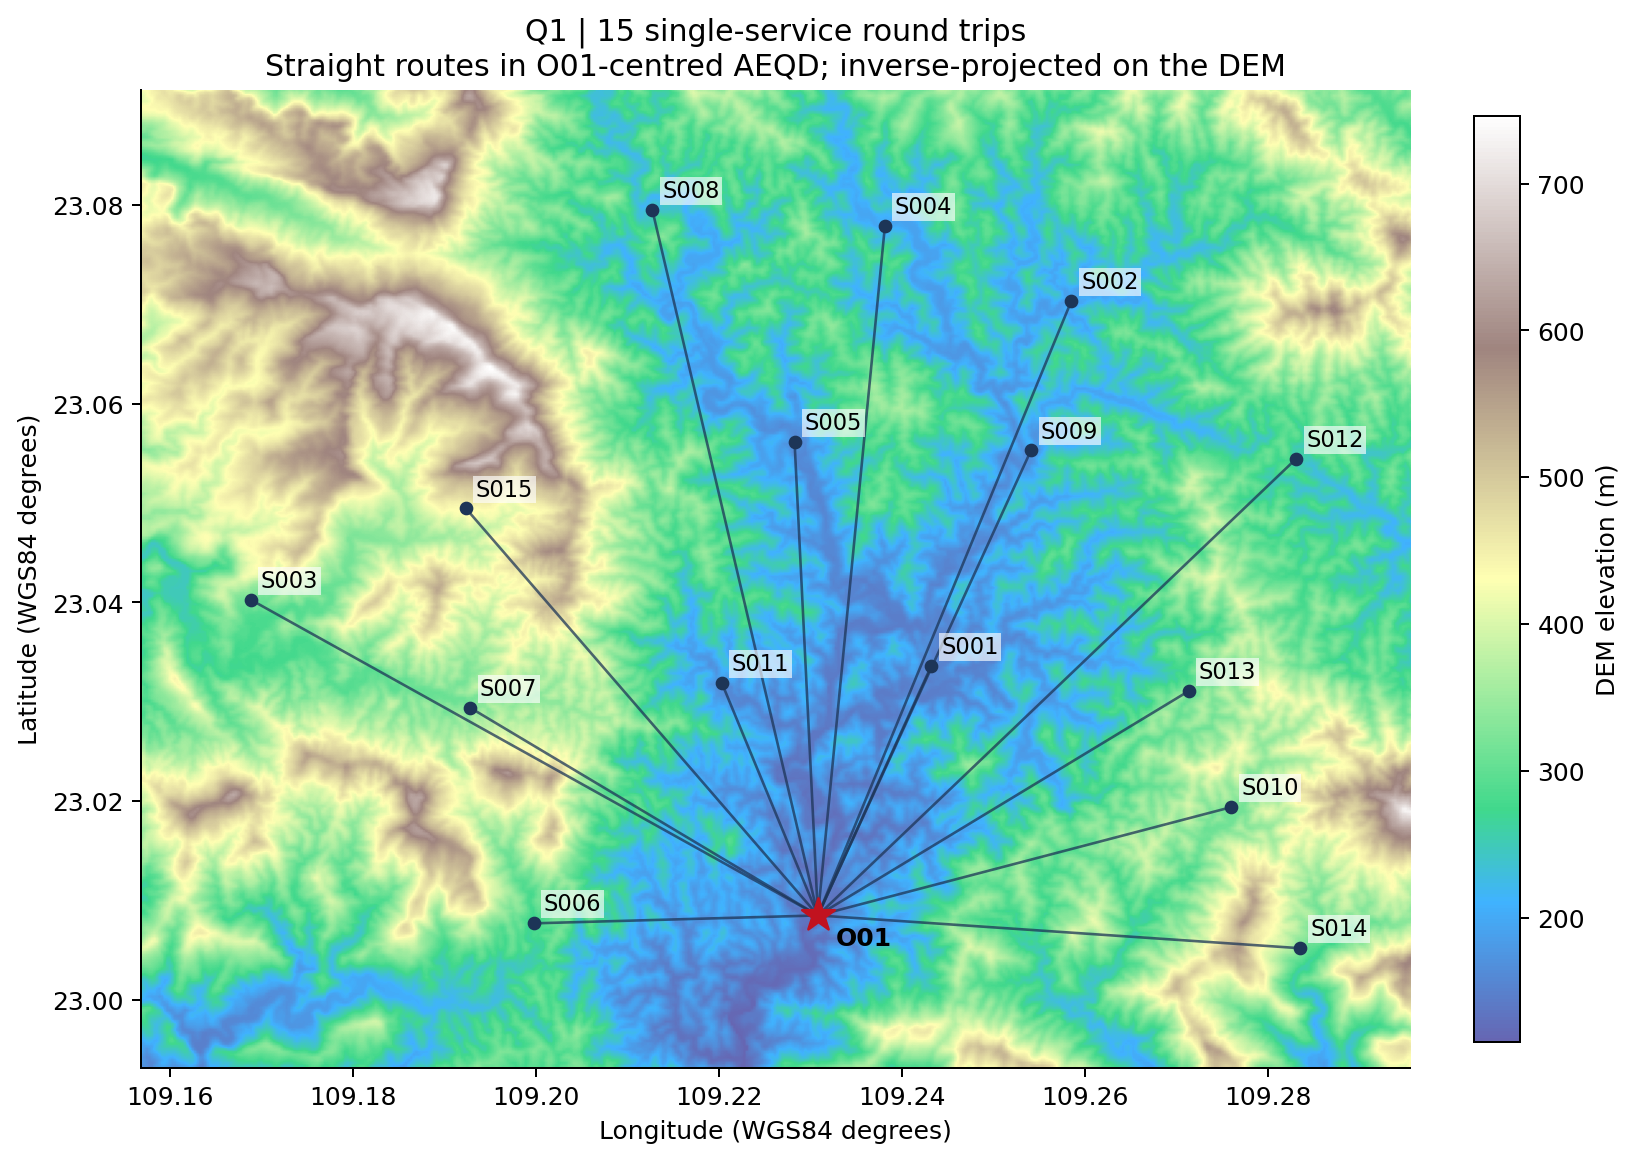
\includegraphics[width=0.82\textwidth]{map_single_routes.png}
  \caption{Q1基地O01至15个服务区的单点往返航线与DEM背景示意。该图仅用于空间关系展示，正式地形计算采用完整DEM像元相交。}
  \label{fig:app_q1_routes}
\end{figure}

\subsection{基线与Pareto结果}

\begin{table}[H]
\centering
\caption{Q1主要基线与正式方案}
\label{tab:app_q1_baseline}
\begin{tabular}{llrrr}
\toprule
机型策略 & 方法 & 架次 & 能耗/kWh & 累计作业时间/min\\
\midrule
A-only & exact & 52 & 112.180153 & 1488.763007\\
B-only & exact & 35 & 68.350657 & 927.625473\\
C-only & exact & 18 & 73.934908 & 563.979235\\
mixed & FFD-mass & 18 & 75.116697 & 563.979235\\
mixed & exact & 18 & \textbf{59.131296} & \textbf{546.266929}\\
\bottomrule
\end{tabular}
\end{table}

完整不同Pareto目标向量仅有两组：
\[
(18,\ 59.131296022053,\ 546.266929148593),
\]
\[
(19,\ 59.033942092203,\ 573.999623452513).
\]

\subsection{改变全局最少架次数的安全余量阈值}

\begin{table}[H]
\centering
\caption{Q1八个全局架次数临界阈值}
\label{tab:app_q1_thresholds}
\begin{tabular}{lcrr}
\toprule
安全余量阈值/\% & 触发区域 & 阈值处架次 & 严格右侧\\
\midrule
23.088350 & S004 & 18 & 19\\
27.049854 & S008 & 19 & 20\\
33.625809 & S008 & 20 & 21\\
33.896918 & S003 & 21 & 22\\
34.373532 & S004 & 22 & 23\\
34.391873 & S002 & 23 & 24\\
34.777897 & S008 & 24 & 25\\
35.267807 & S008 & 25 & 不可行\\
\bottomrule
\end{tabular}
\end{table}

完整569个候选事件与19次词典序最优代表变化由 \path{problems/D/q1/results/reserve_thresholds.csv} 和 \path{problems/D/q1/results/reserve_optimal_segments.csv} 保存。

% ============================================================
\section{问题二任务构造、调度结果与认证证据}
\label{app:q2}

\subsection{23个正式运输任务}

表\ref{tab:app_q2_tasks}直接对应 \path{q2_final/solution/main_23/decisions.json}。任务编号T01--T23仅用于论文展示，原始箱号保持不变。

\scriptsize
\begin{longtable}{cllp{8.2cm}}
\caption{Q2正式23个运输任务构成}\label{tab:app_q2_tasks}\\
\toprule
任务 & 机型 & 访问顺序 & 原始货箱ID\\
\midrule
\endfirsthead
\toprule
任务 & 机型 & 访问顺序 & 原始货箱ID\\
\midrule
\endhead
T01 & C & S001 & S001-MED-01, S001-MED-02, S001-WAT-06, S001-WAT-07, S001-WAT-08, S001-FOD-03, S001-HYG-01, S001-HYG-02\\
T02 & C & S001 & S001-WAT-02, S001-WAT-03, S001-WAT-04, S001-WAT-05, S001-FOD-02\\
T03 & B & S010 & S010-MED-01, S010-WAT-01, S010-FOD-01\\
T04 & B & S014 & S014-MED-01, S014-WAT-01, S014-FOD-01\\
T05 & B & S012 & S012-MED-01, S012-WAT-01, S012-FOD-01\\
T06 & A & S001 & S001-WAT-01, S001-FOD-01\\
T07 & A & S004 & S004-WAT-01, S004-FOD-01\\
T08 & A & S013 & S013-WAT-01, S013-FOD-01\\
T09 & A & S011$\rightarrow$S004 & S004-MED-01, S004-WAT-02, S011-MED-01\\
T10 & C & S006 & S006-MED-01, S006-WAT-01, S006-WAT-02, S006-WAT-03, S006-FOD-01, S006-HYG-01\\
T11 & C & S002 & S002-MED-01, S002-WAT-02, S002-WAT-03, S002-WAT-04, S002-FOD-01, S002-FOD-02, S002-HYG-01\\
T12 & C & S007$\rightarrow$S003 & S003-WAT-02, S003-WAT-03, S003-WAT-04, S003-FOD-01, S003-FOD-02, S003-HYG-01, S007-HYG-01\\
T13 & C & S005 & S005-MED-01, S005-WAT-01, S005-WAT-02, S005-WAT-03, S005-FOD-01, S005-HYG-01\\
T14 & A & S009$\rightarrow$S002$\rightarrow$S013 & S002-WAT-01, S009-MED-01, S013-MED-01\\
T15 & A & S007 & S007-MED-01, S007-WAT-01\\
T16 & A & S007 & S007-WAT-02, S007-FOD-01\\
T17 & B & S004 & S004-WAT-03, S004-HYG-01\\
T18 & B & S008 & S008-MED-01, S008-WAT-01, S008-FOD-01\\
T19 & B & S008 & S008-WAT-02, S008-HYG-01\\
T20 & A & S003$\rightarrow$S015 & S003-MED-01, S003-WAT-01, S015-MED-01\\
T21 & A & S015 & S015-WAT-01, S015-FOD-01\\
T22 & A & S009 & S009-WAT-01, S009-FOD-01\\
T23 & A & S011 & S011-WAT-01, S011-FOD-01\\
\bottomrule
\end{longtable}
\normalsize

\subsection{正式主方案与22架次见证}

\begin{table}[H]
\centering
\caption{Q2正式23架次方案与22架次可行见证}
\label{tab:app_q2_22_23}
\begin{tabular}{lrr}
\toprule
指标 & 正式23架次 & 22架次见证\\
\midrule
A/B/C架次 & 11/6/6 & 11/4/7\\
加权迟到/s & 0 & 0\\
makespan/s & 5693.231489 & 7767.058323\\
总能耗/kWh & 66.214460 & 66.323024\\
最紧硬截止余量/s & 202.096058 & 645.017134\\
最低返航SOC/\% & 20.097383 & 20.097383\\
\bottomrule
\end{tabular}
\end{table}

22架次方案只证明“22架次可行”，不证明22架次的最小makespan，也不能据此推出所有22架次方案均慢于23架次主方案。

\subsection{V7全局有效上下界}

\begin{table}[H]
\centering
\caption{Q2-EVIDENCE-V7-FOCUSED认证摘要}
\label{tab:app_q2_v7}
\begin{tabular}{lr}
\toprule
证据项 & 数值\\
\midrule
全局有效下界/s & 5433.956428\\
认证可行上界/s & 5693.231490\\
区间宽度/s & 259.275062\\
UB归一化间隙 & 4.554093092\%\\
互补分支数 & 809\\
叶证书数 & 810\\
完整机型定价调用 & 2430\\
审计失败数 & 0\\
原问题makespan全局最优 & 未证明\\
\bottomrule
\end{tabular}
\end{table}



\subsection{有限邻域与计算层负结果}

围绕当前主方案共检查330个定向局部邻域，329个有限模型返回不可行，1个达到时限后保持未知；不能将该结果解释为原问题局部或全局最优证明。pricing dominance实验只评价固定真实定价输入：24个输入的各组中位耗时之和由6.323099 s降至2.026581 s，比值为3.1201；生成标签由5,706,982降至2,061,175，最小约化成本保持一致。该3.1201倍不是整个Q2求解器速度比。

% ============================================================
\section{问题三运输--中继联合方案与验证}
\label{app:q3}

\subsection{当前正式release摘要}

当前正式版本为 \texttt{Q3-BOTTLENECK-V6/time}，物理模型版本为 \texttt{Q3-HOVER-COMPATIBLE-V5}。

\begin{table}[H]
\centering
\caption{Q3 V6正式主方案摘要}
\label{tab:app_q3_summary}
\begin{tabular}{lr}
\toprule
指标 & 数值\\
\midrule
运输架次 & 23\\
中继架次 & 4\\
实体运输无人机 & 8\\
运输电池 & 14\\
中继无人机 & 2\\
中继能源组件 & 3\\
联合最后返航/s & 5836.969929\\
运输能耗/kWh & 66.251280\\
中继能耗/kWh & 2.688136\\
总能耗/kWh & 68.939416\\
加权迟到 & 0\\
硬迟到箱数 & 0\\
最小硬截止余量/s & 360.866938\\
最低运输返航SOC/\% & 20.097383\\
\bottomrule
\end{tabular}
\end{table}

\subsection{中继转场高度口径}

中继转场采用
\[
H_R(p)=\max\left\{\max_{c\in\mathcal C(O01,p)}Z(c)+50,\ z_p,\ z_{O01}\right\}.
\]
该规则只作用于中继往返转场，普通运输航段仍使用沿线最高地形+50 m。旧release中将悬停高度额外截断在地形净空巡航面以下，因此其有限候选域证书不能自动继承到V6。

\subsection{连续通信验证}

V6主方案重新构造真实运输轨迹、完整中继需求区间与临界端点。主验证器完成17,756项物理、资源、区间和端点检查，失败0；独立时空点核验36,672点，未发现断链。保存证据包含700份完整区间证书和1,238份临界端点证书。

\subsection{关键保障切换}

关键C型运输任务在V5中从相对956.973974 s起必须依赖西侧中继；V6将此前段保障延长至1039.150288 s，同时使西侧中继提前5.821245 s就绪。两项共同解释约87.997559 s的同模型工期改善。该分析解释保存日程中的关键链，不构成原问题全局下界。

\subsection{时间--能耗与鲁棒备选}

\begin{table}[H]
\centering
\caption{Q3 V6已验证候选}
\label{tab:app_q3_robust}
\begin{tabular}{lrrr}
\toprule
方案 & 额外统一损耗/dB & 联合工期/s & 总能耗/kWh\\
\midrule
time & 0 & 5836.969929 & 68.939416\\
energy & 0 & 5911.548135 & 68.735791\\
robust025 & 0.25 & 5866.140527 & 69.031751\\
q4\_tradeoff & 0 & 5866.140527 & 68.975497\\
\bottomrule
\end{tabular}
\end{table}

旧+0.50/+0.55 dB结果属于历史release，不属于V6；当前只把+0.25 dB方案作为V6下完整核验的通信裕度备选。

% ============================================================
\section{问题四V6严格分区与资源向量}
\label{app:q4}

\subsection{严格模型不可拆块}

冻结Q3 V6/time任务、绝对时刻和实际通信保障关系后，严格模型形成
\[
B_1=\{S001\},\qquad
B_2=\{S002,S003,S004,S005,S007,S008,S009,S010,S011,S012,S013,S014,S015\},\qquad
B_3=\{S006\}.
\]
严格两组共有3种无标签分区，严格三组只有1种。

\subsection{当前正式资源向量}

\begin{table}[H]
\centering
\caption{Q4 V6严格分类型资源需求与库存}
\label{tab:app_q4_vectors}
\begin{tabular}{lrrrr}
\toprule
资源类型 & 原库存 & 全局共享 & 严格K2 & 严格K3\\
\midrule
A型运输机 & 4 & 4 & 4 & 5\\
B型运输机 & 2 & 2 & 2 & 2\\
C型运输机 & 2 & 2 & 3 & 5\\
A型电池 & 6 & 6 & 6 & 7\\
B型电池 & 4 & 4 & 4 & 4\\
C型电池 & 4 & 4 & 4 & 6\\
中继无人机 & 2 & 2 & 2 & 2\\
中继能源组件 & 6 & 3 & 3 & 3\\
\midrule
总配置 & 30 & 27 & 28 & 34\\
\bottomrule
\end{tabular}
\end{table}

严格两组的正式需求和缺口为
\[
\mathbf D^{(2)}=(4,2,3,6,4,4,2,3),\qquad
\boxed{\mathbf G^{(2)}=(0,0,1,0,0,0,0,0)}.
\]
严格三组的需求和缺口为
\[
\mathbf D^{(3)}=(5,2,5,7,4,6,2,3),\qquad
\boxed{\mathbf G^{(3)}=(1,0,3,1,0,2,0,0)}.
\]

两组正式分区为“除S006外14区 / S006”，总缺口1；三组唯一分区为“S001 / 其余13区 / S006”，总缺口7。

\subsection{跨问折中}

V6另保留一个 \texttt{q4\_tradeoff} 候选：联合工期5866.140527 s、总能耗68.975497 kWh，其严格三组缺口为6。它在Q3时间--能耗二维上不优于正式time方案，但说明Q3最短工期与Q4最少独立配置并不等价。

\subsection{历史敏感性边界}

旧Q4-SENSITIVITY-V2中的relay-copy、N-1、Pareto和库存敏感性使用旧Q3日程，未针对V6重新计算。它们仍保留在仓库历史目录，但不能与当前V6 strict资源向量混用。

\subsection{资源最小数量的交叉核验}

对固定任务组和固定资源类型，最小资源数量
\[
N_{gp}^{\min}=\max_t n_{gp}(t)
\]
由事件扫描和半开区间峰值计算得到，并在V6完整运行包中以实体资源链和独立最大匹配进行交叉核验。

% ============================================================

\section{复现、版本锁与证据清单}
\label{app:repro}

\subsection{正式版本入口}

\begin{table}[H]
\centering
\caption{四问正式结果入口}
\label{tab:app_release}
\begin{tabular}{lll}
\toprule
问题 & 正式版本/提交 & 论文复现入口\\
\midrule
Q1 & \texttt{f905acc8482966c...} & \path{problems/D/q1/}\\
Q2 & Q2-EVIDENCE-V7-FOCUSED & \path{problems/D/q2/evidence_v7/}\\
Q3 & Q3-BOTTLENECK-V6 / time & \path{problems/D/q3/release_v6/time/}\\
Q4 & Q4-STRICT-FROM-Q3-V6 & \path{problems/D/q4/results_q3_v6/}\\
\bottomrule
\end{tabular}
\end{table}

\subsection{哈希锁定的伴随归档}

\begin{longtable}{p{6.5cm}p{8.0cm}}
\caption{正式伴随归档SHA-256}\label{tab:app_archives}\\
\toprule
归档 & SHA-256\\
\midrule
\endfirsthead
\toprule
归档 & SHA-256\\
\midrule
\endhead
D题\_Q2定向证据强化V7\_源码证书与复核.zip &
\texttt{0804f989699dc506b3111dacc7408d9acdeb6e1115e7f32ec36934116de6ce58}\\
D题\_Q3正式封口\_FINAL\_源码结果与交接.zip &
\texttt{97f5ea8018a557d604bee87d6886675ecf7648f035e8df0f47f20ff6e7fbc56b}\\
D题\_Q4稳健性完善V2\_源码结果与验证.zip &
\texttt{9c8d1a6410c2de0a410318fc3525dc162613deabf4ba9dd1d59cdeb98437f5b4}\\
D题\_Q2外部方案复核\_代码明细与验证.zip &
\texttt{b41a0416313a123e734e01d7ca1672b99acee41f16edd79812302e1007610b77}\\
\bottomrule
\end{longtable}

\subsection{证据等级与最终提交前检查}

正式论文中只允许使用与证据强度相匹配的表述：
\begin{itemize}
  \item Q1最少18架次：原Q1模型下全局证明；
  \item Q2加权迟到0：第一层目标全局证明；
  \item Q2 makespan：有效全局下界与完整可行上界，未闭合；
  \item Q3 V6：连续区间/临界端点与独立重放证明保存方案完整可行；
  \item Q3固定结构：连续时间LP证明当前固定离散结构下的时序最优；
  \item Q3鲁棒性：仅$+0.25$ dB为当前V6完整可行见证，旧$+0.50/+0.55$ dB不继承；
  \item Q4 K2/K3：冻结Q3 V6/time日程后的strict完整分区枚举。
\end{itemize}

最终提交前应再次以 \path{paper_integration/FINAL_SELECTION.json} 为唯一选择入口，逐项核对正文、摘要、图表、附录和机器可读结果，避免旧版本数字残留。


\end{document}
